%\documentclass{book}\usepackage{sjtfonts}\usepackage{includegraphics}\usepackage{alltt}\usepackage{latexsym}
%\usepackage{array}
%\begin{document}\input{defs0}%		miradefs.tex 		    June 1994

% opening and closing a quoted Miranda section

\newcommand{\mira}{\noindent\hrulefill\nopagebreak\so}
\newcommand{\arim}{\nopagebreak\st\hrulefill\\}

% backslash in the Miranda environment
% Only feasible approach is to use \verb+\+
% in line!

%\newcommand{\bs}{$\mi\backslash\!\!$}
%\newcommand{\lbs}{\mbox{\verb+\+}}

% ignoring part of the input

\newcommand{\ignore}[1]{}

% a blank line in a Miranda section

\newcommand{\bl}{\mbox{\ }}

% Signalling a diffculty.

\definecolor{light-gray}{gray}{0.95}

\newcommand{\beware}[2]
 {\medskip\noindent\colorbox{light-gray}{\parbox{\textwidth}
 {\mbox{\large\textbf{#1}} \medskip\noindent\\ #2}\medskip\noindent}}

% Subscripting in Miranda text
\newcommand{\subscr}[2]{\mbox{${\mbox{\texttt{#1}}}_{\mbox{\texttt{#2}}}$}}

%\newcommand{\subscr}[2]{\mbox{${\mbox{\mi #1}}_{\mbox{\smtt #2}}$}}
\newcommand{\aone}{\subscr{a}{1}}
\newcommand{\atwo}{\subscr{a}{2}}
\newcommand{\ak}{\subscr{a}{k}}

\newcommand{\aoneone}{\subscr{a}{1,1}}

\newcommand{\eone}{\subscr{e}{1}}
\newcommand{\etwo}{\subscr{e}{2}}
\newcommand{\ei}{\subscr{e}{i}}
\newcommand{\er}{\subscr{e}{r}}

\newcommand{\fone}{\subscr{f}{1}}
\newcommand{\fl}{\subscr{f}{l}}

\newcommand{\gone}{\subscr{g}{1}}
\newcommand{\gtwo}{\subscr{g}{2}}
\newcommand{\gi}{\subscr{g}{i}}
\newcommand{\gr}{\subscr{g}{r}}

\newcommand{\hone}{\subscr{h}{1}}
\newcommand{\hl}{\subscr{h}{l}}

\newcommand{\pone}{\subscr{p}{1}}
\newcommand{\ptwo}{\subscr{p}{2}}
\newcommand{\pk}{\subscr{p}{k}}

\newcommand{\qone}{\subscr{q}{1}}
\newcommand{\qtwo}{\subscr{q}{2}}
\newcommand{\qk}{\subscr{q}{k}}

\newcommand{\rone}{\subscr{r}{1}}
\newcommand{\rtwo}{\subscr{r}{2}}

\newcommand{\tone}{\subscr{t}{1}}
\newcommand{\ttwo}{\subscr{t}{2}}
\newcommand{\tn}{\subscr{t}{n}}

\newcommand{\vone}{\subscr{v}{1}}
\newcommand{\vtwo}{\subscr{v}{2}}
\newcommand{\vn}{\subscr{v}{n}}

% for regular expressions

\newcommand{\stone}{\subscr{st}{1}}
\newcommand{\sttwo}{\subscr{st}{2}}
\newcommand{\stn}{\subscr{st}{n}}
\newcommand{\rthree}{\subscr{r}{3}}

\newcommand{\eps}{$\varepsilon$}
\newcommand{\trans}[1]{\stackrel{\mbox{\tt #1}}{\longrightarrow}}



% superscript in Miranda text

\newcommand{\superscr}[2]{\mbox{${\mbox{\mi #1}}^{\mbox{\smtt #2}}$}}

% Not equals in Miranda text

\newcommand{\noteq}{\makebox[0pt][l]{=}/}
\newcommand{\overslash}{\makebox[0pt][l]{/}}

% Definitions in complexity chapter

\newfont{\oldSym}{cmsy10}
\newcommand{\Th}{\boldmath$\oldSym\Theta$}
\newcommand{\pow}[1]{\^{}#1}
\newcommand{\leqq}{$\leq$}
\newcommand{\geqq}{$\geq$}
\newcommand{\lll}{$\ll$}
\newcommand{\eqq}{$\equiv$}
\newcommand{\ltwo}{\subscr{log}{2}}

% Indexing

\newcommand{\minx}[1]{\index{#1@{\ttfamily{}#1}}}
\setcounter{chapter}{9}\setcounter{page}{157}


\chapter{Higher-order functions}
\chapstart
\label{gen2}
\index{higher-order function}

Haskell is a \emph{functional} programming language: that means that the main way in which we compute things is by defining functions which describe how to transform the inputs into the required output. Haskell has a collection of built-in data types which we can use to model the data in the problem domain, including numbers, booleans, lists, tuples and \texttt{data} types.

Haskell is also functional in a more distinctive way: \emph{functions are data} in Haskell, and can be treated just like data of any other type. \index{function!as data}
\begin{itemize}
\item
Functions can be combined using \emph{operators}, just like the numbers can be combined using the arithmetical operators.
\item
Haskell provides \emph{lambda abstractions}, which allow us to describe functions directly by expressions, rather than having to define and name a function in order to use it.
\item
Functions can be the inputs and outputs of other functions in exactly the same way as any other type. Functions which have other functions as arguments or results are called \emph{higher-order functions}.
\item
In particular, the syntax of Haskell makes it particularly easy to \emph{partially apply} functions and operators, so that functions are returned as the results of applying functions.
\end{itemize}
This chapter covers these topics, setting the scene for Chapter \ref{developingHOPs} where will put these ideas into practice.

Finally, we'll also see that we can start to write function-level definitions -- sometimes called `point-free' definitions -- which can be more concise, more readable and more suitable for program verification and transformation. Indeed, the chapter concludes with
some examples of program verification involving higher-order polymorphic
functions, and we see there that the theorems proved about them are reusable in
exactly the same way that the functions themselves are reusable.


\section{Operators: function composition and application}

This section describes the built-in operators for function composition and application, as well as defining a new operator, forward composition, which composes functions in the `natural' order.

\subsection*{Function composition: \texttt{.}}
\index{function composition|(}

\begin{figure}[t]
\begin{center}
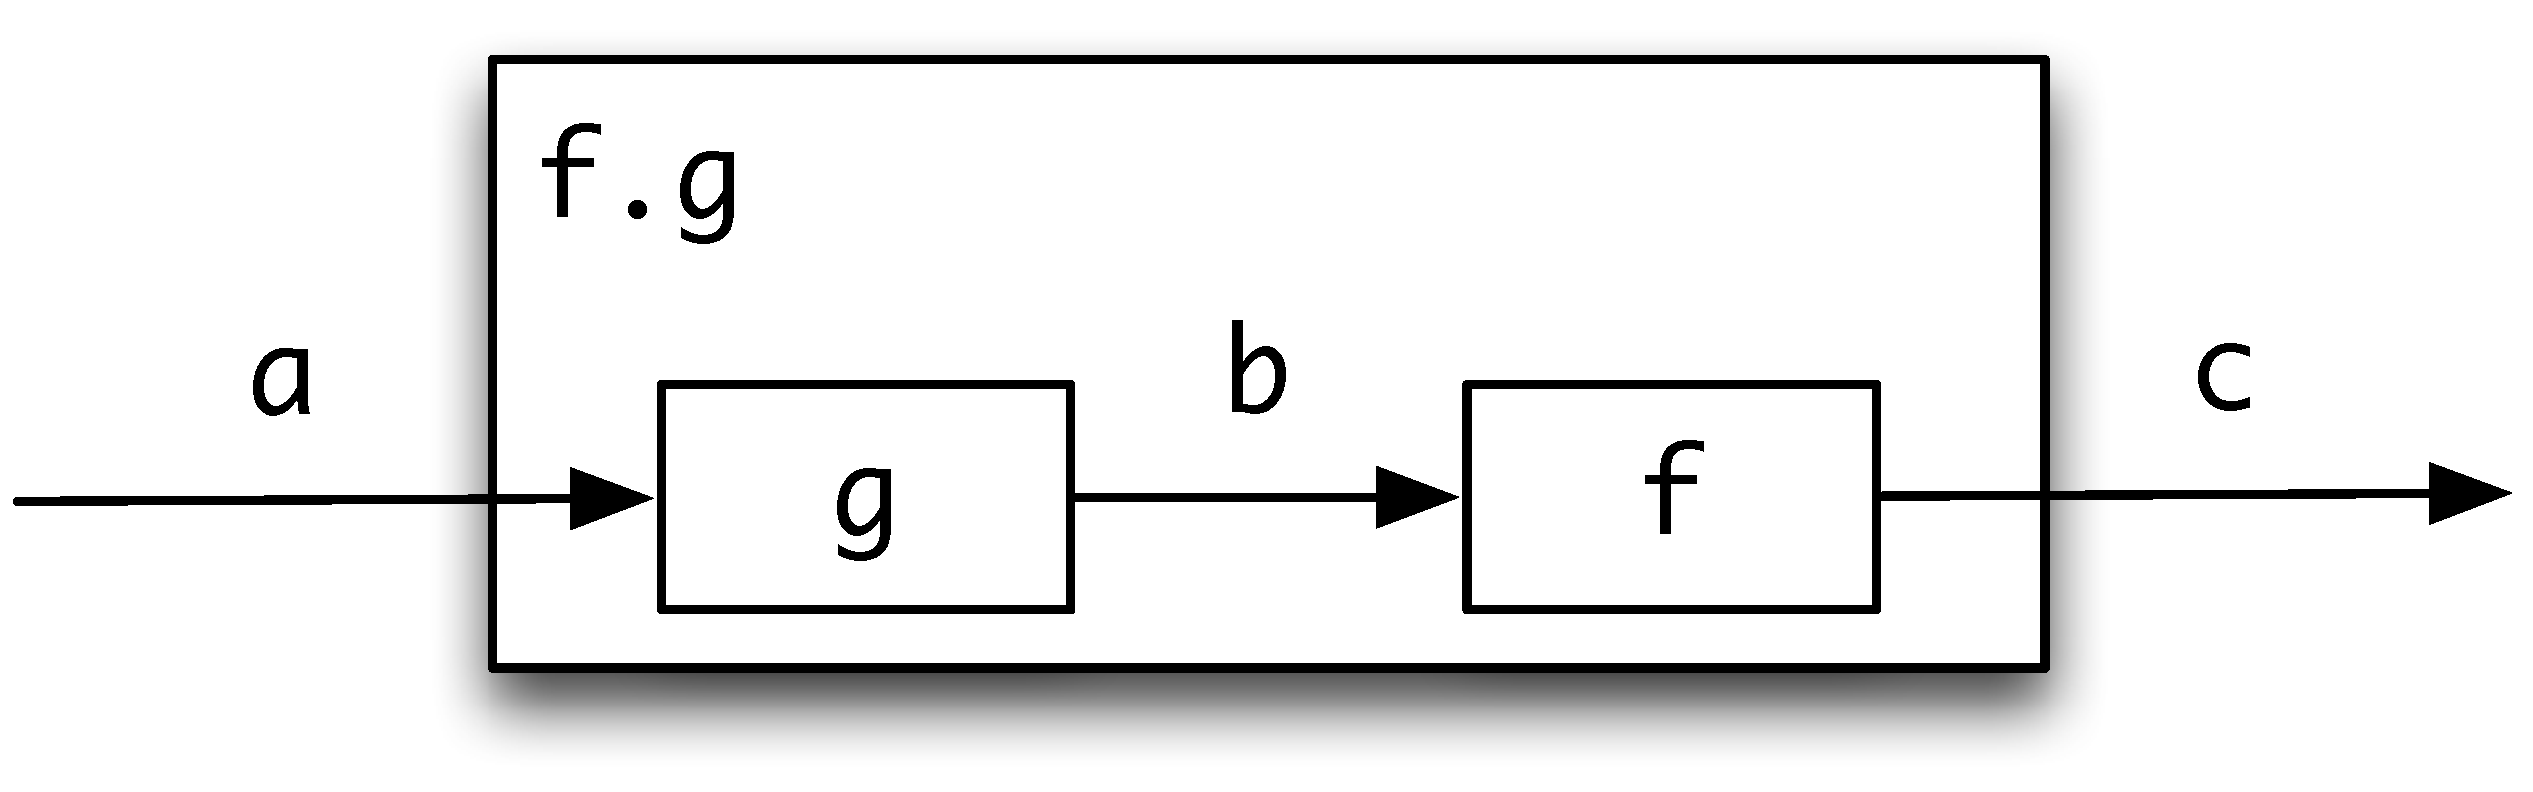
\includegraphics[width=3in]{Pictures/compos.pdf}
\end{center}
\caption{Function composition}
\label{funComp}
\end{figure}

Function composition is one of the simplest ways of structuring a program: do a number of things
one after the other: each part can be designed and implemented separately. 

Haskell has the \textbf{function composition}  operator over functions built in. The operator, which is denoted by the `\texttt{.}' between the two functions, has the effect of `wiring together' two functions: passing the output of one to the input of another, and it is .  This is pictured in Figure \ref{funComp}, where the annotations of the arrows in the diagram
indicate the types of elements involved.


For any functions \texttt{f} and \texttt{g}, the effect of \texttt{f.g} is given by
the definition
\begin{alltt}
(f.g) x = f (g x)\hfill(comp.1)
\end{alltt}
Not all pairs of functions can be composed. The output of \texttt{g}, \texttt{g x},
becomes the input of \texttt{f}, so that the output type of \texttt{g} must equal
the input type of \texttt{f}. 

Recalling the \texttt{Picture} example, we have already seen a definition of \texttt{rotate}:
\begin{alltt}\minx{rotate}
rotate :: Picture -> Picture
rotate pic = flipV (flipH pic)\hfill(rotate.1)
\end{alltt}
Using the composition operator we can say directly that \texttt{rotate} is the composition of \texttt{flipH} with \texttt{flipV}:
like
\begin{alltt}
rotate = flipV . flipH\hfill(rotate.2)
\end{alltt}
Notice that we explained the definition \texttt{(rotate.2)} as the `composition of \texttt{flipH} with \texttt{flipV}': why that way round? We do this because \texttt{flipH} is the function that is applied first, with \texttt{flipV} being applied to the result of the first application. We are able to compose \texttt{flipH} with \texttt{flipV} because the output of
\texttt{flipH} and the input of \texttt{flipV} are both of 
\texttt{Picture} type.



In general, the constraint on which functions can be composed 
is expressed by giving `\texttt{.}' the type
\begin{center}
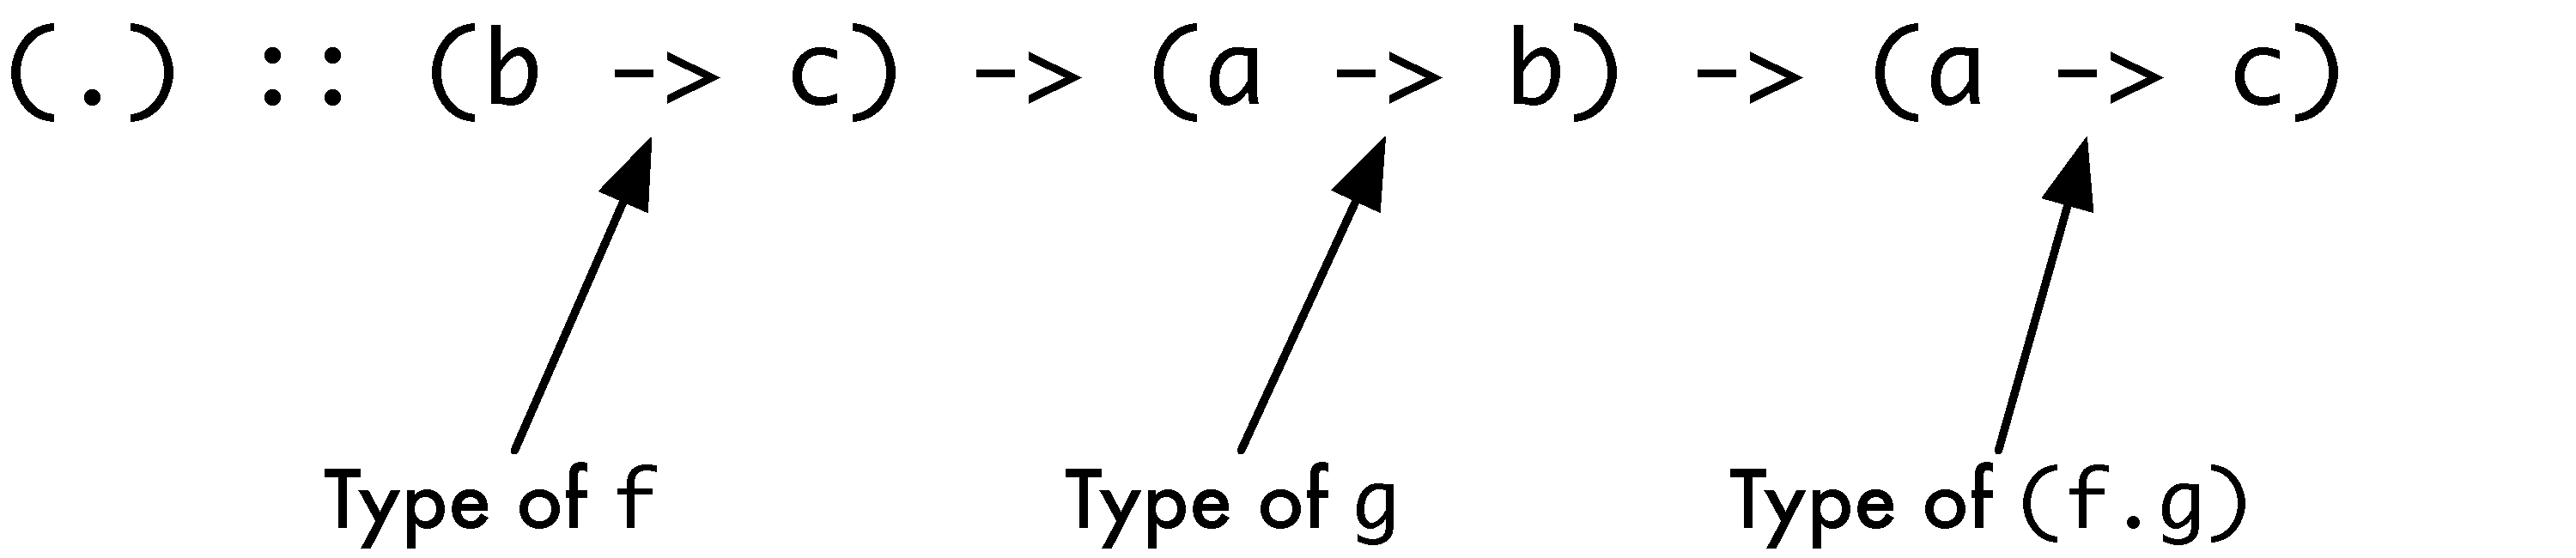
\includegraphics[width=3.5in]{Pictures/composType.pdf}
\end{center}\index{function composition!type of}
which shows that, if we call the first input \texttt{f} and the second \texttt{g}, 
\begin{titemize}
\item The input of \texttt{f} and the output of \texttt{g} are of the same type: 
\texttt{b}.
\item The result \texttt{f.g} has the same input type, \texttt{a}, as \texttt{g} and 
the same output type, \texttt{c}, as \texttt{f}.
\end{titemize}
Composition is {\bf associative}, that is \index{associativity}
\texttt{f.(g.h) } is equal to \texttt{(f.g).h} for all \texttt{f}, \texttt{g} and 
\texttt{h}. We can therefore write \texttt{f.g.h} unambiguously to mean `do \texttt{h}, then
\texttt{g}, then \texttt{f}'.\footnote{For technical reasons, the `\texttt{.}'
is treated as right associative in the Haskell standard prelude.}


\begin{figure}[t]\index{function composition!binding power of}
\beware{The `binding power' of composition}{
There is a common error caused by the binding powers of
function application and function composition. 

It is an error to write \texttt{f.g x} thinking it
means \texttt{(f.g)} applied to \texttt{x}. Because function application binds more
tightly than anything else, it is interpreted by the system
as \texttt{f.(g x)}, which will often lead to a type
error. 
For example, evaluating 
\begin{alltt}
not.not True
\end{alltt}
gives the type error message
\begin{alltt}
\ \ \ \ Couldn't match expected type `a -> Bool'

\ \ \ \ \ \ \ \ \ \ \ \ against inferred type `Bool'

\ \ \ \ In the second argument of `(.)', namely `not True'

\ \ \ \ In the expression: not . not True

\ \ \ \ In the definition of `it': it = not . not True
\end{alltt}
since there is an attempt to treat \texttt{not True} as a function to be composed
with \texttt{not}. Such a function needs to have type \texttt{a -> Bool}, 
whereas it actually has type \texttt{Bool}. 

In applying a composition we therefore need to be sure that it is
\textbf{parenthesized} like this:
\begin{alltt}
(not.not) True
\end{alltt}
}
\end{figure}


\subsection*{Forward composition: \texttt{>.>}}
\index{forward composition}
\index{function composition!forward}

The order in \texttt{f.g} is significant, and can be confusing; \texttt{(f.g)}
means `first apply \texttt{g} and then apply \texttt{f} to the result', so the function that is applied first comes second in the composition.


It is simple in Haskell to define an operator for composition which takes its
arguments in the opposite order to `\texttt{.}', like this:
\begin{alltt}\index{\symbol{62}\symbol{46}\symbol{62}@\texttt{\symbol{62}\symbol{46}\symbol{62}}}
infixl 9 >.>
\bl
(>.>) :: (a -> b) -> (b -> c) -> (a -> c)
\bl
g >.> f = f . g\hfill(fcomp.1)
\end{alltt}
This definition has the effect that
\begin{alltt}
(g >.> f) x = (f.g) x = f (g x)\hfill(fcomp.2)
\end{alltt}
showing that, as it were, the order of the \texttt{f} and \texttt{g} is swapped
before the functions are applied.
The \texttt{rotate} example can then be written
\begin{alltt}\minx{rotate}
rotate = flipH >.> flipV  
\end{alltt}
which we can read as \texttt{flipH} {\em then\/} \texttt{flipV}, with the
functions being applied \emph{from left to right}. 

The notation `\texttt{>.>}' contains a `\texttt{.}' to show that it is a form of
composition, with the arrows showing the direction in which information is
flowing. We will tend to use `\texttt{>.>}' in situations where a number
of functions are composed, and it is therefore tiresome to read some
lines down the page in order to work out the effect of a function
definition.





\index{function composition|)}

\subsection*{The application operator: \texttt{\$}}\minx{\$}\index{application operator (\texttt{\$})}

We're familiar in Haskell with how to write the application of a function \texttt{f} to an argument \texttt{e}: we just write \texttt{f} next to \texttt{e}, like this: \texttt{f e}. In other words, we \textbf{juxtapose} the function and its argument.

We can also explicitly write down an application using the application operator, `\texttt{\$}', like this: \texttt{f \$ e}. Why on earth would we want to do this, when we can write it without the `\texttt{\$}'? There are two reasons that an explicit application gets used:
\begin{itemize}
\item
Many Haskell programmers use `\texttt{\$}' as an alternative to parentheses, so you may well see this in libraries that people have written. 
Instead of writing something like
\begin{alltt}
flipV (flipH (rotate horse))
\end{alltt}
it is possible to write:
\begin{alltt}
flipV $ flipH $ rotate horse
\end{alltt}
with the same meaning. Arguably this is a little clearer, and it is shorter! Incidentally you can see from this example that `\texttt{\$}' is \textbf{right associative}.
\item
We need to use the application operator as a function, as in the example
\begin{alltt}
zipWith ($) [sum,product] [[1,2],[3,4]] 
\end{alltt}
where the application operator is applied to corresponding elements of the two lists.\end{itemize}

\begin{figure}[t]\index{application operator (\texttt{\$})!and composition}\index{function composition!and application (\texttt{\$})}
\beware{Application and composition}{
Application and composition can get confused. Function composition combines two functions,
while application combines a function and an argument (which can be a
function, of course).
\itempar
If, for example, 
\texttt{f} has type \texttt{Integer -> Bool}, then
\begin{itemize}
\item[--]
\texttt{f.x} means \texttt{f} composed with the {\em function\/} \texttt{x}; \texttt{x}
therefore needs to be of type \texttt{s~->~Integer} for some type \texttt{s}.  
\item[--]
\texttt{f x} means \texttt{f} applied to the object \texttt{x}, so \texttt{x} must
therefore be an integer.
\item[--]
\texttt{f \$ x} also means \texttt{f} applied to the object \texttt{x}, and so \texttt{x} must
again be an integer.
\end{itemize}
}
\end{figure}




\begin{exercises}

\item
Redefine the function \texttt{printBill} from the supermarket billing exercise
in Section \ref{superBill} so that composition is used. Repeat the exercise using
forward composition, \texttt{>.>}.

\item
If \texttt{id} is the polymorphic identity function, defined by 
\texttt{id x = x}, explain the
behaviour of the expressions 
\begin{alltt}
(id.f)         (f.id)         id f
\end{alltt}If \texttt{f} is of type
\texttt{Int -> Bool}, at what instance of its most general type \texttt{a -> a}
is \texttt{id} used in each case? What type does
\texttt{f} have if \texttt{f id} is properly typed?

\item
Define a function \texttt{composeList} which composes a list of
functions into a single function. You should give the
type of \texttt{composeList}, and explain why the function has this
type. What is the effect of your function on an empty list of functions?


\item
What is the type of the application operator, \texttt{\$}?

\item
What is the result of the expression given above:
\begin{alltt}
zipWith ($) [sum,product] [[1,2],[3,4]] 
\end{alltt}

\item
If \texttt{id} is the polymorphic identity function, defined by 
\texttt{id x = x}, explain the
behaviour of the expressions 
\begin{alltt}
(id \$ f)         (f \$ id)         id (\$)
\end{alltt}If \texttt{f} is of type
\texttt{Int -> Bool}, at what instance of its most general type \texttt{a -> a}
is \texttt{id} used in each case? What type does
\texttt{f} have if \texttt{f \$ id} is properly typed?





\end{exercises}



\section{Expressions for functions: lambda abstractions}
\label{exprFuns}

Haskell definitions give us a way of defining functions, and once we have defined a function we can use its name to refer to it, as in the application
\begin{alltt}
map addOne [2,3,4]
\end{alltt}
assuming that we've already defined
\begin{alltt}
addOne x = x+1
\end{alltt}
Haskell gives us a way of writing down an expression that means `the function that adds one to a number' directly, without having to give it a name. We write
\begin{alltt}
\bs{}x -> x+1
\end{alltt}
which we can read as saying `the function  that takes \texttt{x} to \texttt{x+1}', the initial `\bs{}' signalling that it's a function. So, we can add one to all the numbers in the list \texttt{[2,3,4]} by writing the expression
\begin{alltt}
map (\bs{}x -> x+1) [2,3,4]
\end{alltt}
An expression like \texttt{(\bs{}x -> x+1)} is called a \emph{lambda abstraction}.\index{lambda abstraction} 

\beware{Why is a called a `lambda abstraction'?}{The `lambda' comes from the lambda calculus, a
mathematical theory of functions. The symbol `\texttt{\bs{}}' is the closest
ASCII character to the Greek character lambda, $\lambda$, used in the $\lambda$-calculus. One of the inventors of the $\lambda$-calculus was Haskell B.\ Curry, after whom Haskell is named. 

The `abstraction' comes from the fact that the expression \texttt{(\bs{x} -> e)} is a function, which `abstracts away' from the particular expression \texttt{e}.}

\subsection*{Examples of lambda abstractions}

Let's take a look at some other uses of this notation now. Suppose that we want to take a list of functions and apply them all to a particular argument,
\begin{alltt}
mapFuns :: [a->b] -> a -> [b]
\end{alltt}
giving a list of results. We might do this in playing a game of Rock - Paper - Scissors  where we apply a number of different strategies to the current game position, and then compare the different results; we'll come back to this scenario later in the chapter.

We could define the function by recursion, like this:
\begin{alltt}
mapFuns [] x     = []
mapFuns (f:fs) x = f x : mapFuns fs x
\end{alltt}
but in fact we can use \texttt{map} in making the definition: what we have to do at each element of the list (remember, each element is a function) is to apply it to \texttt{x}, so
\begin{alltt}
mapFuns fs x = map (\bs{}f -> f x) fs
\end{alltt}
What's important to see here is that the function \texttt{(\bs{}f -> f x)} depends on the  value of \texttt{x}, and so we cannot define it as a top level function. We could, alternatively, define it in a \texttt{where} clause,
\begin{alltt}
mapFuns fs x = map applyToX fs
			   where
			   applyToX f = f x
\end{alltt}
The first definition is clearer, and defines the operative function directly, rather than having to name and define it in a \texttt{where} clause, separately from where it is used; of course, either is OK, and it's a matter of taste which you might use.  

One of the main uses of lambda abstractions is to define functions which are the results of functions. Let's look at the example of the function
\begin{alltt}
addNum :: Integer -> (Integer -> Integer)
\end{alltt}
The function takes an integer, 17 say, and returns a function: in this case the function that adds 17 to its argument. The definition says this directly:
\minx{->}\minx{addNum}
\begin{alltt}
addNum n = (\bs{m} -> n+m)
\end{alltt}

\subsection*{`Plumbing' functions together}

Another example which uses a lambda abstraction is given by the
`plumbing' illustrated in Figure \ref{plumb}.
\begin{figure}[t]
\begin{center}
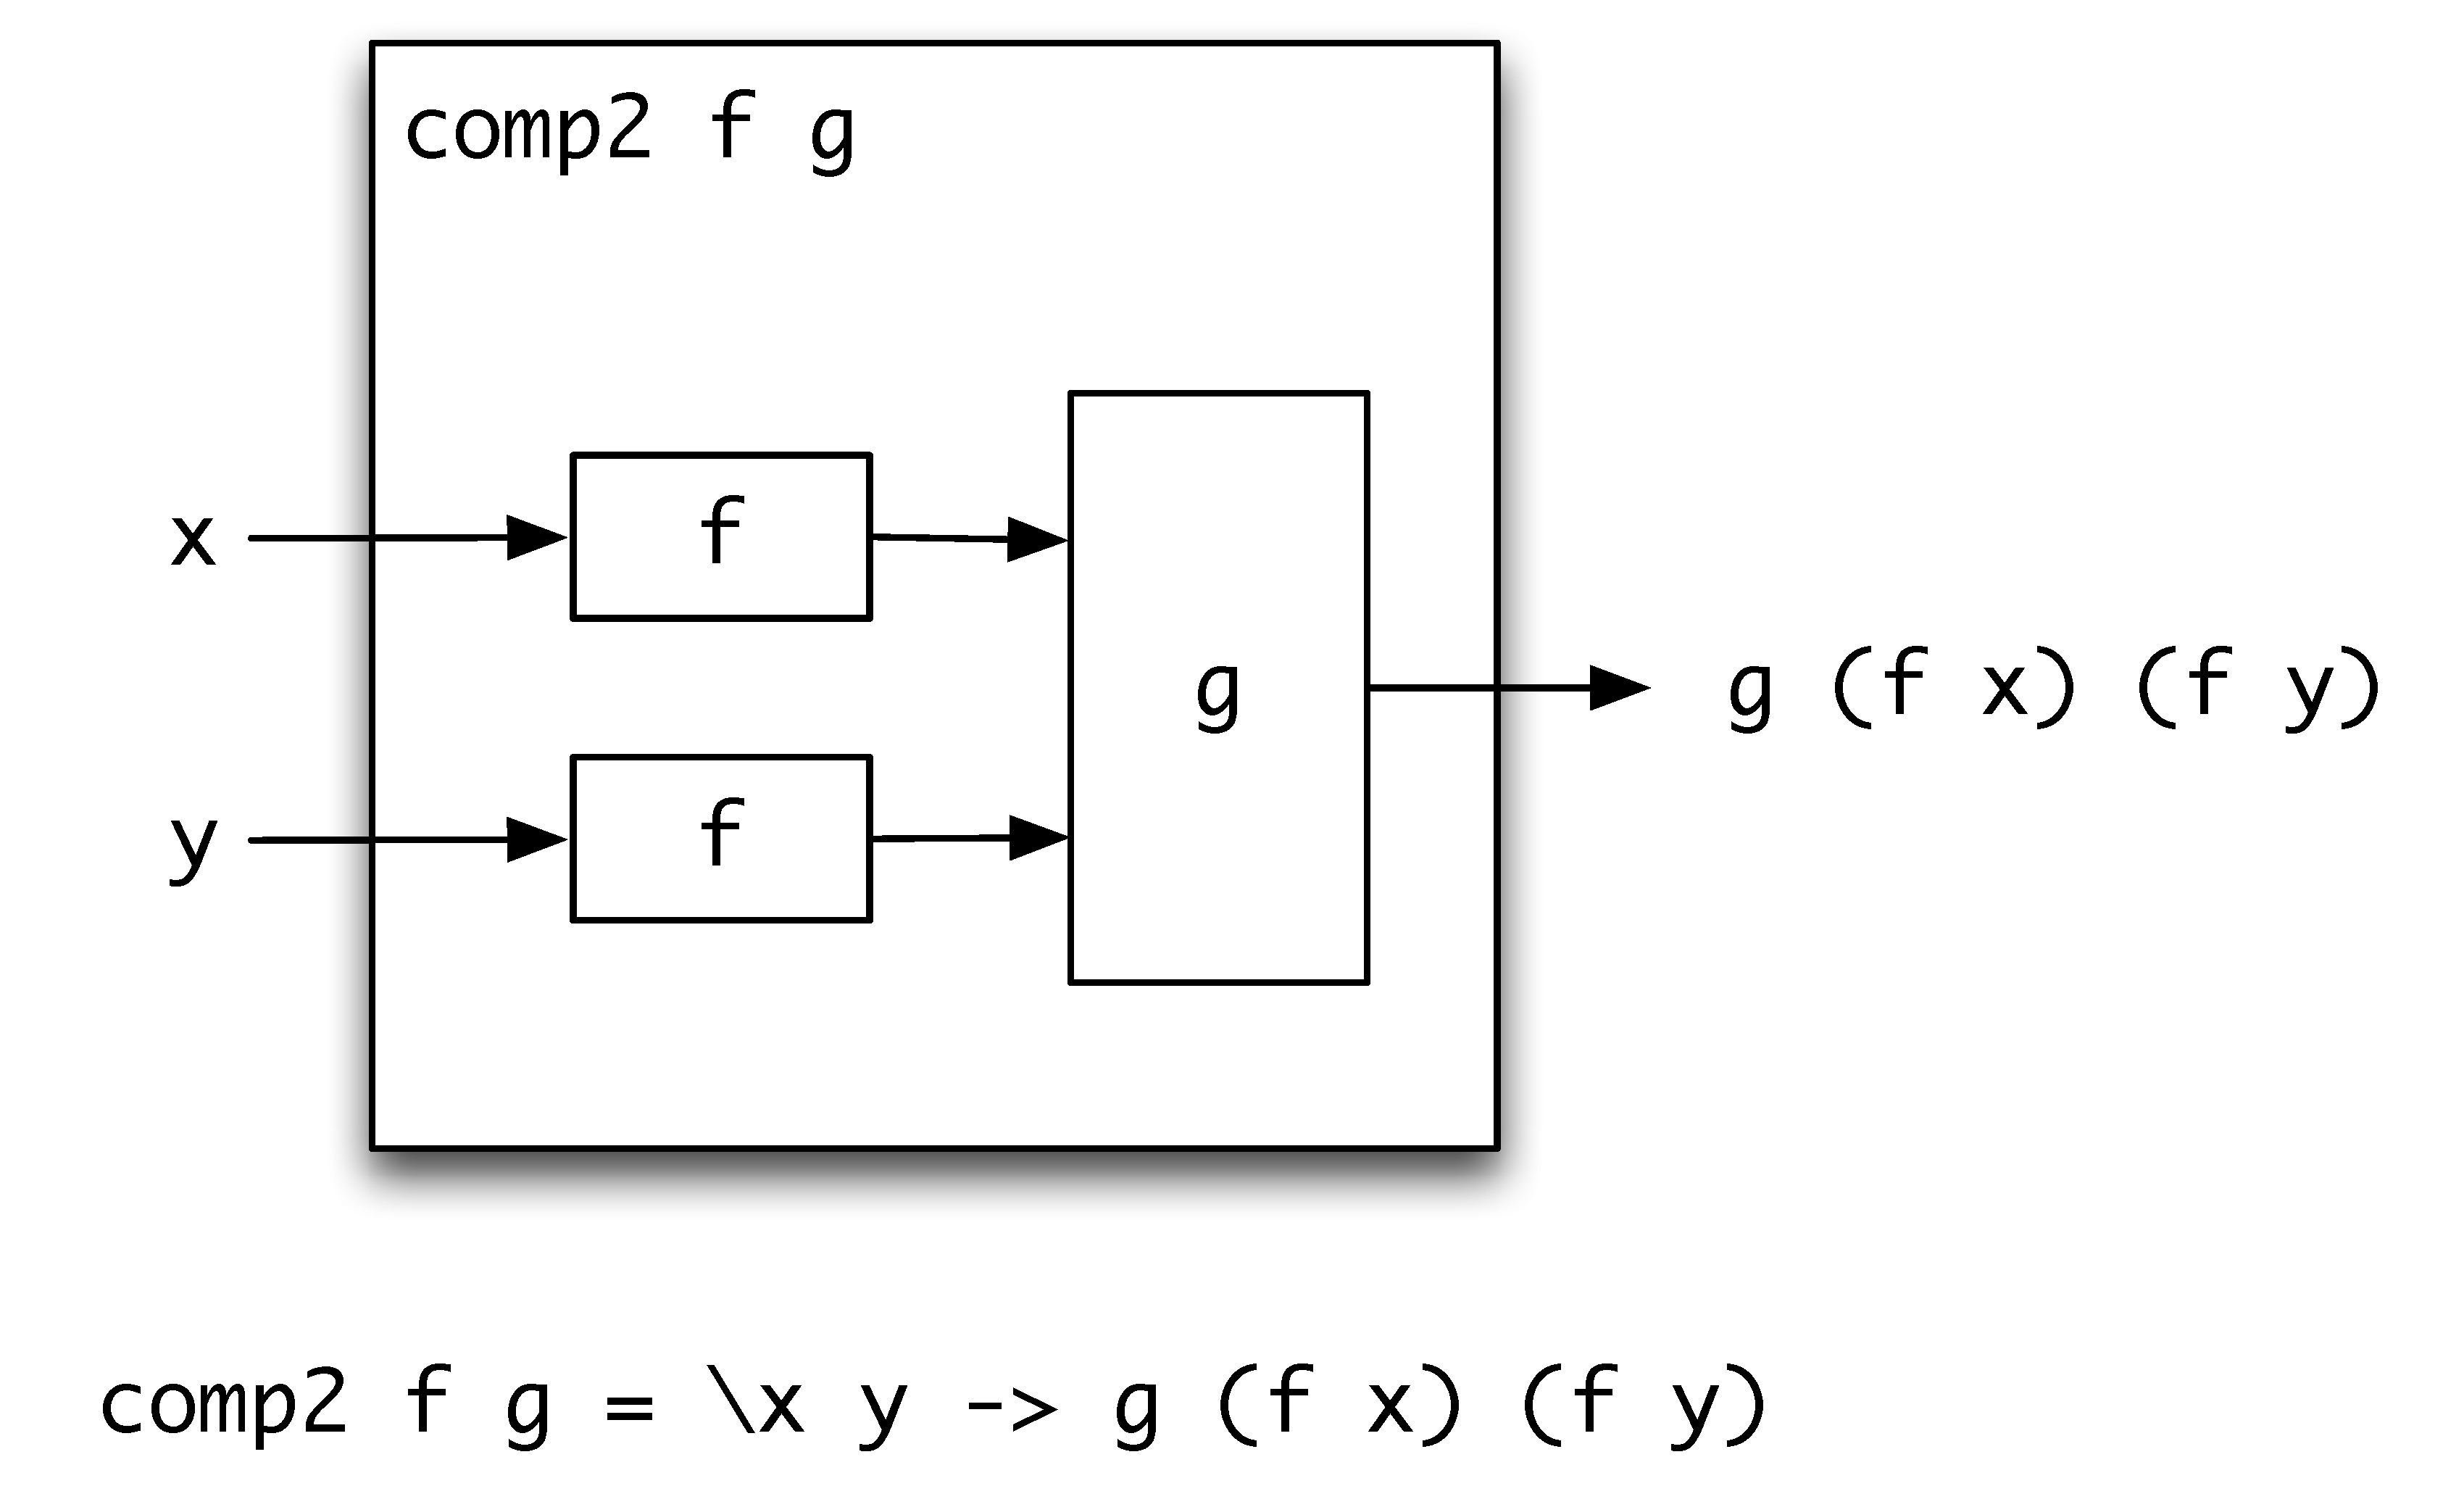
\includegraphics[width=4in]{Pictures/comp2.pdf}
\end{center}
\caption{Plumbing \texttt{f} and \texttt{g} together.}
\label{plumb}\index{plumbing}
\end{figure}
The object shown
is a function, whose arguments are \texttt{x} and \texttt{y}. The result 
of the function is 
\begin{alltt}
g (f x) (f y)
\end{alltt}
so the overall effect is to give a
function which applies \texttt{f} to each of its (two) arguments before applying
\texttt{g} to the results. Again, the definition states this directly:
\begin{alltt}\minx{comp2}
comp2 :: (a -> b) -> (b -> b -> c) -> (a -> a -> c)
\bl
comp2 f g = (\bs{x} y -> g (f x) (f y))
\end{alltt}
To add together the squares of \texttt{3} and \texttt{4} we can write
\begin{alltt}
comp2 sq add 3 4
\end{alltt}
where \texttt{add} and \texttt{sq} have the obvious definitions.

In general, a lambda abstraction is an \textbf{anonymous}
version\index{function!anonymous}
of the sort of function we have defined earlier. In other words, the
function \texttt{f} defined by
\begin{alltt}
f x y z = result
\end{alltt}
and the function
\begin{alltt}
\bs{}x y z -> result
\end{alltt}
have exactly the same effect.

We shall see in the next
section that partial application will make many definitions -- including some
of the functions here -- more straightforward. On the other hand the
lambda abstraction is more general, and thus can be used in situations when
a partial application could not.

\begin{exercises}

\item
Using a lambda abstraction, the Boolean function \texttt{not}
and the built-in function \texttt{elem}
describe a function of type
\begin{alltt}
{\hskip1pc}Char -> Bool
\end{alltt}
which is \texttt{True} only on non-whitespace characters, that is those which are
not elements of the list \texttt{" \bs{t}\bs{n}"}.

\item
Define a function \texttt{total}
\begin{alltt}
{\hskip1pc}total :: (Integer -> Integer) -> (Integer -> Integer)
\end{alltt}
so that \texttt{total f} is the function which at value \texttt{n} gives the total
\begin{alltt}
{\hskip1pc}f 0 + f 1 + \ldots + f n
\end{alltt}
You should be able to do this using built-in functions, rather than using recursion.

\item
Given a function \texttt{f} of type \texttt{a -> b -> c}, write down a lambda abstraction that
describes
the function of type \texttt{b -> a -> c} which behaves like \texttt{f} but
which takes its arguments in the other order. Pictorially,
\begin{center}
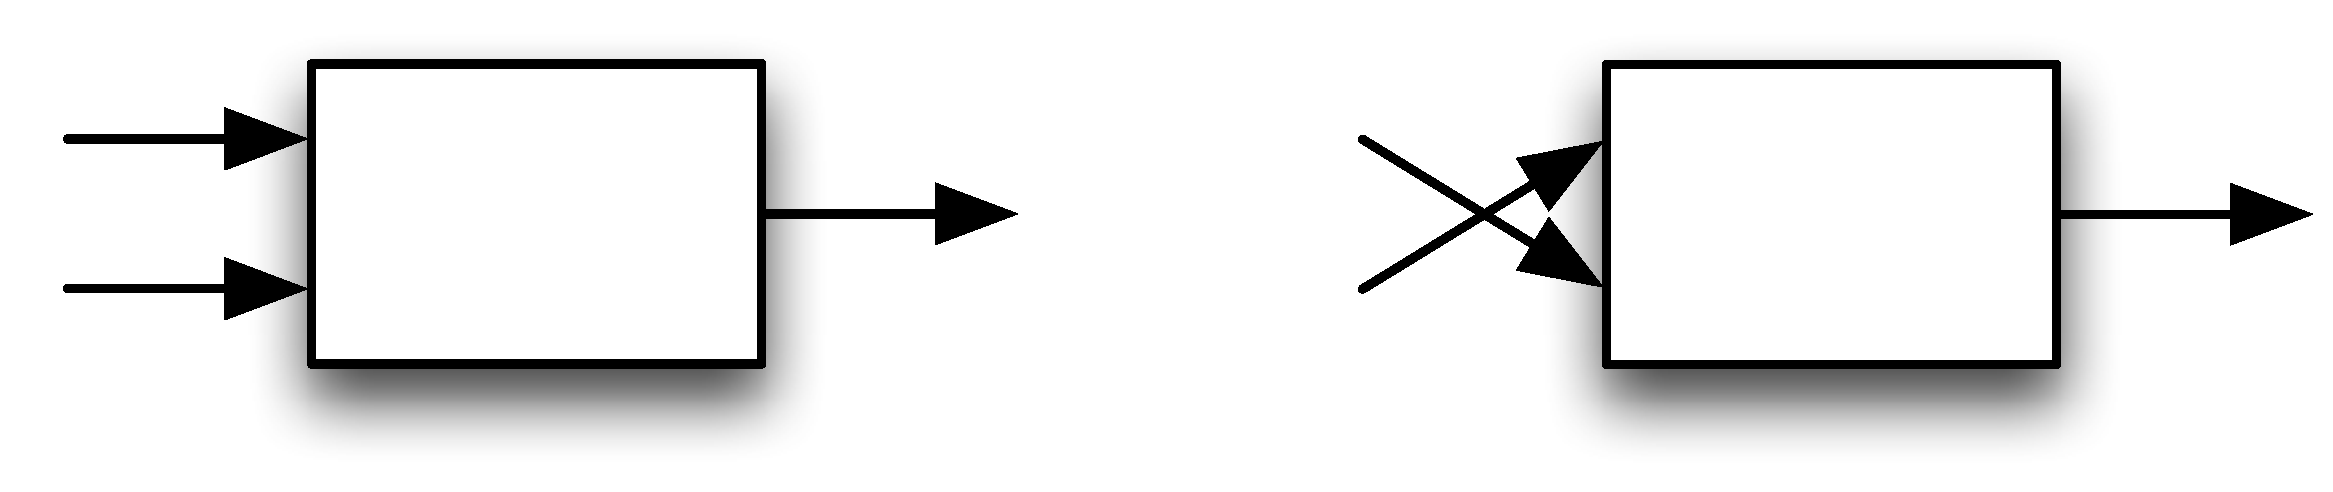
\includegraphics[width=3.4in]{Pictures/flip.pdf}
\end{center}


\item
Using the last exercise, or otherwise, give a definition of the function
\begin{alltt}
{\hskip1pc}{\hskip1pc}flip :: (a -> b -> c) -> (b -> a -> c)
\end{alltt}
which reverses the order in which its function argument takes its arguments.


\end{exercises}







\section{Partial application}\index{partial application|(}
\index{function application!partial|see{partial application}}


In this section we'll discover how it is possible to \emph{partially apply} functions in Haskell, and what the effect of this is. Underlying the Haskell approach to functions is what is called the \emph{curried} representation of functions, in honour of Haskell Curry; this is introduced in the section after this. 

\subsection*{Introducing partial application}


The function \texttt{multiply} multiplies together two arguments,
\begin{alltt}
multiply :: Int -> Int -> Int\minx{multiply}
multiply x y = x*y
\end{alltt}
We can view the function as a box, with two input arrows and an output arrow.
\begin{center}
\mbox{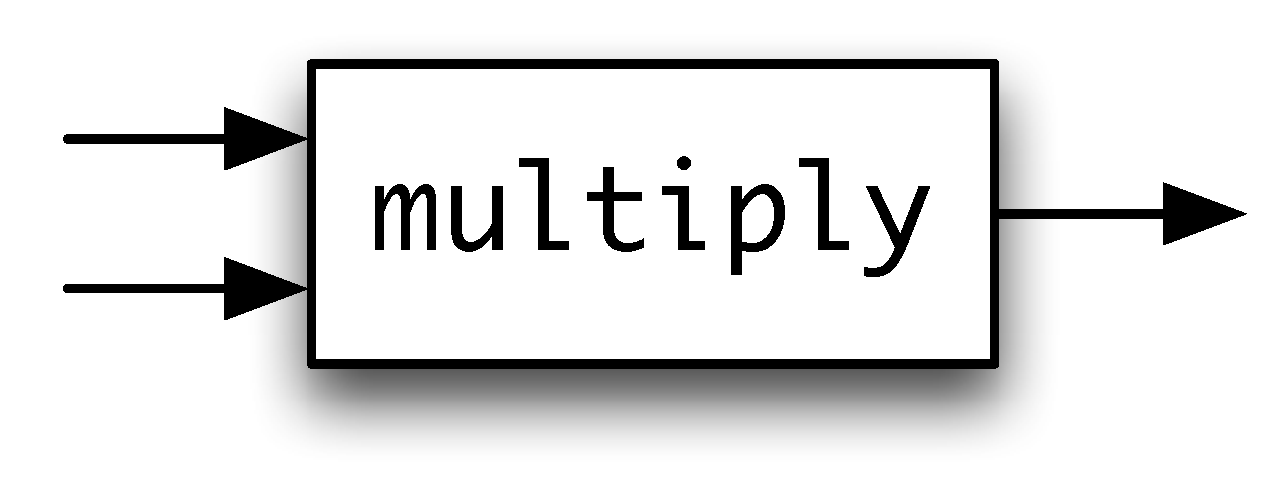
\includegraphics[height=1.5cm]{Pictures/mult1.pdf}}
\end{center}
If we apply the function to two arguments, the result is a number;
so that, for instance, \texttt{multiply 2 3} equals \texttt{6}. 
\begin{center}
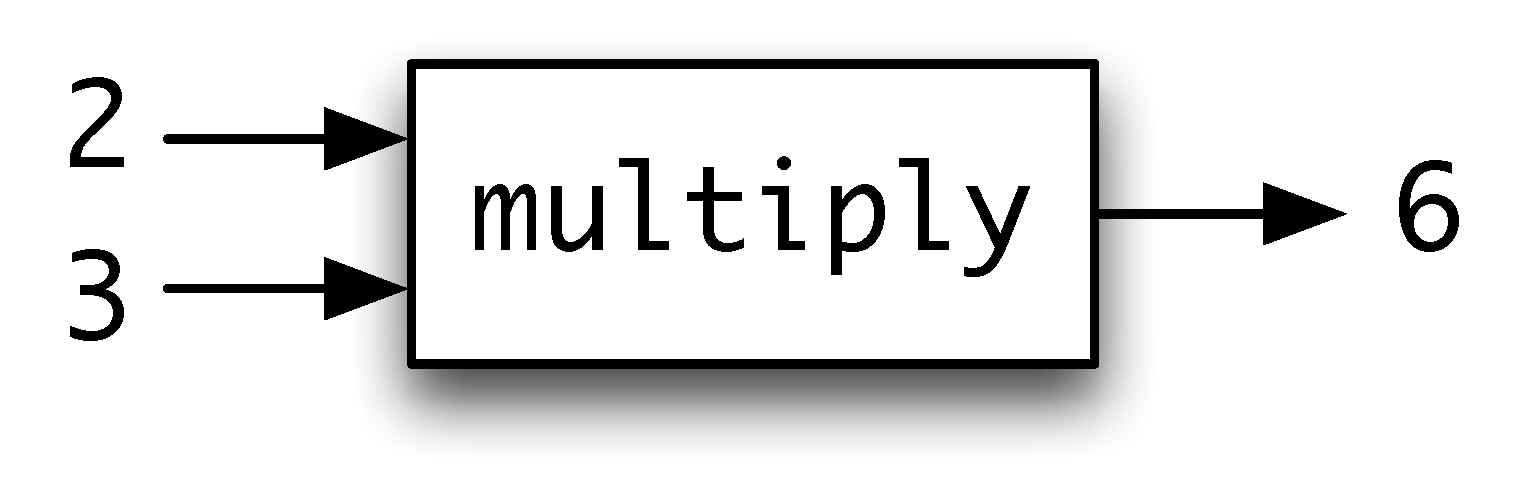
\includegraphics[height=1.5cm]{Pictures/mult2.pdf}
\end{center}
What happens if \texttt{multiply} is
applied to \textbf{one} argument \texttt{2}? Pictorially, we have
\begin{center}
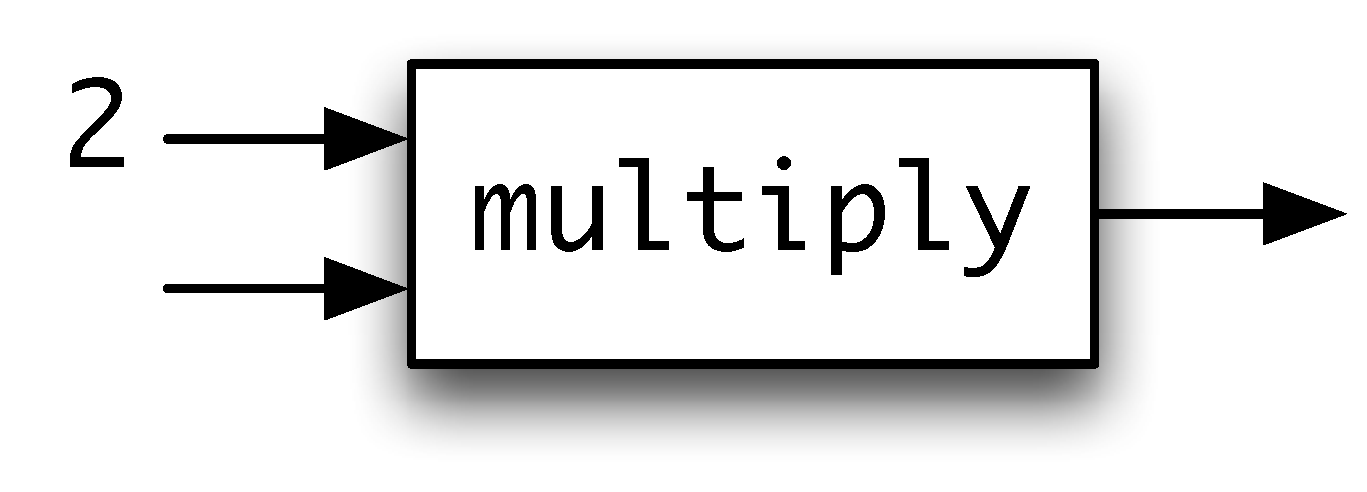
\includegraphics[height=1.5cm]{Pictures/mult3.pdf}
\end{center}
From the picture we can see that this represents a function, as there is 
still one input arrow to the function awaiting a value. This function 
will, when given the awaited argument \texttt{y}, return double its value, namely \texttt{2*y}.

This is an example of a general phenomenon: any function taking two or more
arguments can be \textbf{partially applied} to one or more arguments. This gives
a powerful way of forming functions as results. 



\subsection*{Example: the \texttt{doubleAll} function}


\noindent
To illustrate, we at the example of the function which doubles every element in a list of integers. The function can be defined like this:
\begin{alltt}
doubleAll :: [Int] -> [Int]\minx{doubleAll}
doubleAll = map (multiply 2)
\end{alltt}
In this definition there are two partial applications:
\begin{titemize}
\item \texttt{multiply 2} is a function from integers to integers, given by
applying \texttt{multiply} to one rather than two arguments;
\item \texttt{map (multiply 2)} is a function from \texttt{[Int]} to \texttt{[Int]},
given by partially applying \texttt{map}.
\end{titemize}
Partial application is being put to two different uses here.
\begin{titemize}
\item In the first case -- \texttt{multiply 2} -- the partial
application is used to form the function which
multiplies by two, and which is passed to \texttt{map} to form
the \texttt{doubleAll} function.
\item the second partial application -- of \texttt{map} to
\texttt{multiply 2} -- could be avoided by writing the argument to \texttt{doubleAll} 
\begin{alltt}
doubleAll xs = map (multiply 2) xs
\end{alltt}
but it is quite possible to write a \emph{function level} definition like this, and it is shorter and clearer than the definition with the arguments supplied.
\end{titemize}
In Section \ref{exprFuns} we saw the example of \texttt{addNum}, 
\begin{alltt}\minx{addNum}
addNum n = (\bs{m} -> n+m)
\end{alltt}
which when applied to an integer \texttt{n}
was intended to return the function which adds \texttt{n} to its
argument. With partial application we have a simpler mechanism, as we
can say
\begin{alltt}
addNum n m = n+m
\end{alltt}
since when \texttt{addNum} is applied to one argument \texttt{n} it returns the 
function adding \texttt{n} to its argument.

\begin{figure}[t]\index{argument!order of arguments}
\beware{Order of arguments}{
It is not always possible to make a partial application, since the argument to
which we
want to apply the function may not be its first argument.
Let's look at the function
\begin{alltt}\minx{elem}
elem :: Char -> [Char] -> Bool
\end{alltt}
We can test whether a character \texttt{ch} is a whitespace character by writing
\begin{alltt}
elem ch whitespace
\end{alltt}
where \texttt{whitespace} is the string
\texttt{" \bs{t}\bs{n}"}. We would like to write the function to test this by
partially applying \texttt{elem} to \texttt{whitespace}, but cannot, because this is the secdon argument rather than the first.

One solution is to define
a variant of \texttt{elem} which takes its arguments in the other order, as in
\begin{alltt}\minx{member}
member xs x = elem x xs
\end{alltt}
and write the function as the partial application 
\begin{alltt}
member whitespace
\end{alltt} 
Alternatively, we can
write down this function as a lambda abstraction, like this:
\begin{alltt}
\bs{ch} -> elem ch whitespace
\end{alltt}
}\end{figure}


\subsection*{Partially applied operators: operator sections}
\index{operator sections}
\label{opsecs}

The operators of the language can be partially applied, giving what are
known as {\bf operator sections}. Examples include

\medskip
\noindent
\begin{mytable}
\ttfamily (+2) & The function which adds two to its argument.\\
\ttfamily (2+) & The function which adds two to its argument.\\
\ttfamily (>2) & The function which returns whether a number is greater
than two.\\
\ttfamily (3:) & The function which puts the number \texttt{3} on the front of a
list.\\
\ttfamily (++"\bs{n}") & The function which puts a newline at the end of a string.\\
\ttfamily ("\bs{n}"++) & The function which puts a newline at the beginning of a string.\\ 
\ttfamily (\$ 3) & The function which applies its argument -- which will have to be a function -- to the integer \texttt{3}.\\ 
\end{mytable}

\medskip
\noindent
The general rule here is that a section of the operator \texttt{op} will put
its argument to the side which completes the application. That is, 
\begin{alltt}
(op x) y = y op x
(x op) y = x op y
\end{alltt}
When combined with higher-order functions like \texttt{map}, 
\texttt{filter} and composition, the notation is both powerful and elegant, 
enabling us to make a whole lot more function-level definitions. For example,
\begin{alltt}
filter (>0) . map (+1)
\end{alltt}
is the function which adds one to each member of a list, and then removes those
elements which are not positive.

\begin{figure}[t]\index{parentheses!different roles in Haskell}
\beware{Parentheses in Haskell}{
The main role of parentheses, \texttt{(} \ldots \texttt{)}, in Haskell is to group items together so that the system interprets what you have written in the right way. Typical examples include
\begin{titemize}
\item
enclosing a pattern in a definition, as in \texttt{sum (Node t1 t2) = \ldots};
\item
enclosing a negative literal in a function application, as in \texttt{fac (-1)};
\item
enclosing a type annotation, as in \texttt{foldr plus (1::Int) [1..1000]};
\item
overriding the binding power of operators, as in \texttt{(2+3)*6};
\item
grouping names in a \texttt{deriving} clause like \texttt{deriving (Eq, Show)
}.
\end{titemize}
However, other uses of parentheses have an effect of building data elements or changing the meaning of an identifier.
\begin{titemize}
\item
To form a tuple, it is necessary to enclose the items in parentheses, as in \texttt{(1,True)}; the notation \texttt{1,True} on its own is meaningless.
\item
To turn an infix operator into a prefix operator, it must be enclosed in parentheses, as in \texttt{(\&\&)}.
\item
To form an operator section, the operator and arguments are enclosed in parentheses as seen in this example: \texttt{(\&\& True).(0 /=).(`rem` 2)}.
\end{titemize}
}
\end{figure}

\subsection*{Using partial applications}

The partial application and operator sections is important in Haskell programming. We have already seen that
many functions can be defined as {\bf specializations} of general operations
\index{specialization}
like \texttt{map}, \texttt{filter} and so on. These specializations arise by
passing a function to the general operation -- this function is often
given by a partial application, as in the examples from the pictures
case study first seen in Chapter \ref{intro}:
\begin{alltt}\minx{flipV}\minx{beside}
flipV  = map reverse
beside = zipWith (++)
\end{alltt}
We return to look at the \texttt{Picture} case study in greater detail
in Section \ref{hofPicture}.

More examples of partial applications will be seen throughout the material to
come, and can be used to simplify and clarify many of the preceding examples.
Three simple examples are the text processing functions we first looked at in Section \ref{textProc}:
\begin{alltt}
dropSpace = dropWhile (member whitespace)\minx{dropSpace}
dropWord  = dropWhile (not .\ member whitespace)\minx{dropWord}
getWord   = takeWhile (not .\ member whitespace)\minx{getWord}
\end{alltt}
where
\begin{alltt}
member xs x = elem x xs
\end{alltt}
 
\begin{exercises}


\item
Use partial applications to define the functions \texttt{comp2} and
\texttt{total} given in Section \ref{exprFuns} and its exercises.

\item
Find operator sections \texttt{\subscr{sec}{1}} and
\texttt{\subscr{sec}{2}} so that
\begin{alltt}
map \subscr{sec}{1} . filter \subscr{sec}{2}
\end{alltt}
has the same effect as
\begin{alltt}
filter (>0) .\ map (+1)
\end{alltt}


\item
Re-define the function \texttt{mapFuns}, first defined in Section \ref{exprFuns}, using an operator section of the application operator, \texttt{\$}.
\end{exercises}

\section{Under the hood: curried functions}

Functions in Haskell are represented in \textbf{curried} form, where they take their arguments one at a time.
This
\index{Curry, Haskell B.}
is called {\bf currying} after Haskell Curry\footnote{In fact the first
person to describe the idea was Sch\"{o}nfinkel, but `Sch\"{o}nfinkeling' does
not sound so snappy!} who was one of the pioneers of 
the $\lambda$-calculus and after whom the Haskell language is named. This section explains how curried functions work, and how we can covert to and fro between curried and uncurried form.

Why are Haskell functions in curried form? A major reason is that it supports partial application, as explored in the previous section; it also gives a `clean' readable form to the syntax. One reason against choosing a curried representation is its unfamiliarity to most programmers; another is discussed towards the end of the section.

\index{partial application|)}

\subsection*{Curried functions and function arguments}
\index{function!number of arguments}

\index{partial application}
Partial application can appear confusing: in some contexts functions appear
to take one argument, and in others more than one. In fact, {\em every function in
Haskell takes exactly one argument}. This is called the \textbf{curried} representation of functions.If this application yields a function,
then this function may be applied to a further argument, and so on.
Consider the multiplication
function again. 
\begin{alltt} 
multiply :: Int -> Int -> Int\minx{multiply}
\end{alltt}
This is shorthand for
\begin{alltt} 
multiply :: Int -> (Int -> Int)
\end{alltt}
and so it can therefore be applied to an integer. Doing this
gives (for example)
\begin{alltt}
multiply 2 :: Int -> Int
\end{alltt}
This can
itself be applied to give
\begin{alltt}
(multiply 2) 5 :: Int
\end{alltt}
which, since function application is left associative, can be written 
\begin{alltt}
multiply 2 5 :: Int
\end{alltt}
Our explanations earlier in the book are consistent with this full explanation
of the system. We hid the fact that
\begin{alltt}
f \eone \etwo \ldots \subscr{e}{k}
\tone -> \ttwo -> \ldots \tn -> t
\end{alltt}
were shorthand for
\begin{alltt}
( \ldots((f \eone) \etwo) \ldots \subscr{e}{k})
\tone -> (\ttwo -> (\ldots(\tn -> t)\ldots))
\end{alltt}
but this did no harm to our understanding of how to use the Haskell
language. It is to support this shorthand that function application is
made left associative and \texttt{->} is made right associative.

\begin{figure}[t]
\beware{The syntax of application and \texttt{->}}{\index{function application!syntax}\index{syntax!of application}Function application is {\bf left associative} so
that
\texttt{f x y} means \texttt{(f x) y}, \emph{not} \texttt{f (x y)}.

\medskip
The function space symbol `\texttt{->}'\minx{->} is {\bf right
associative}, so that \texttt{a -> b -> c} means
\texttt{a~->~(b~->~c)}, \emph{not}
\texttt{(a~->~b)~->~c}.}
\end{figure}

\begin{figure}[t]\index{associativity!arrow not associative}
\beware{The arrow is not associative.}{Functions \texttt{f ::\ Int -> Int -> Int} and 
\texttt{g ::\ (Int -> Int) -> Int} are illustrated here
\begin{center}
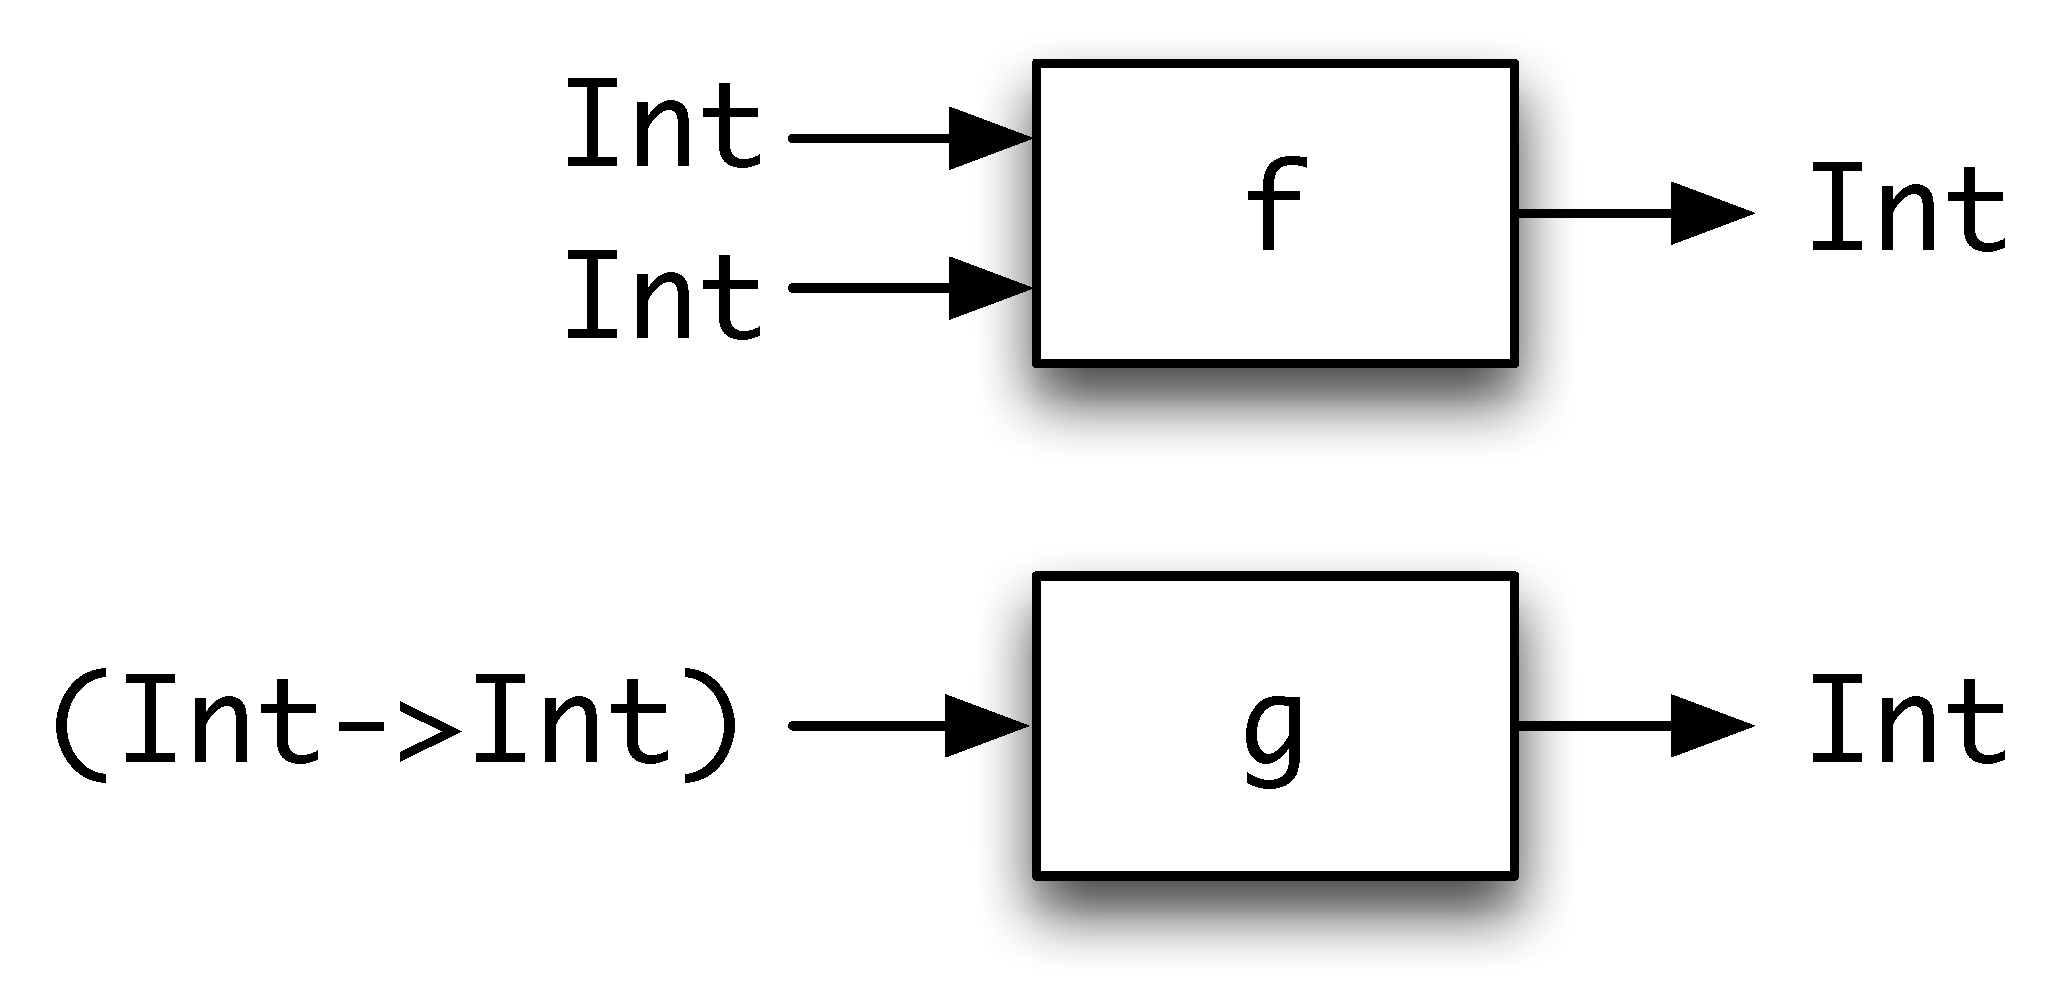
\includegraphics[width=3.0in]{Pictures/arrowDiags.pdf}
\end{center}
The function \texttt{f} will yield a
function from \texttt{Int} to \texttt{Int} when given a \texttt{Int} -- an example is
\texttt{multiply}. 
On the other hand,
when given a function of type \texttt{Int -> Int},
\texttt{g} yields a \texttt{Int}.
An example is
\begin{alltt}
g :: (Int -> Int) -> Int

g h = (h 0) + (h 1)
\end{alltt}
The function \texttt{g} defined here takes a function \texttt{h} as argument and
returns the sum of \texttt{h}'s values at \texttt{0} and \texttt{1}, and
so \texttt{g succ} will have the value \texttt{3}.
}\end{figure}

\subsection*{The types of partial applications}
\index{partial application!type of}

How is the type of a partial application determined? There
is a simple rule which explains it.

\begin{definition}{%
{\sffamily Rule of cancellation}
\medskip

\index{type checking!rule of cancellation}

\begin{quote}
If the type of a function \texttt{f} is
\begin{alltt}
{\hskip1pc}\tone -> \ttwo -> ... -> \tn -> t
\end{alltt}
and it is applied to arguments
\begin{alltt}
{\hskip1pc}\eone::\tone, \etwo::\ttwo, \ldots, \subscr{e}{k}::\subscr{t}{k}
\end{alltt}
(where$\;$\texttt{k$\leq$n})$\;$then$\;$the$\;$result$\;$type$\;$is$\;$given$\;$by$\;${\bf cancelling}$\;$the$\;$types$\;$\texttt{\tone}$\;$to~\subscr{t}{k}

\begin{alltt}
{\hskip1pc}\makebox[0pt][l]{/}\tone -> \makebox[0pt][l]{/}\ttwo -> ... -> \makebox[0pt][l]{/}\subscr{t}{k}-> \subscr{t}{k+1} -> ... -> \tn -> t
\end{alltt}
which gives the type
\begin{alltt}
{\hskip1pc}\subscr{t}{k+1} -> \subscr{t}{k+2} -> ... -> \tn -> t
\end{alltt}\end{quote}}
\end{definition}


\noindent
For example, using this rule we can see that we get the following types
\begin{alltt}
multiply 2      :: Int -> Int
multiply 2 3    :: Int
doubleAll       :: [Int] -> [Int]
doubleAll [2,3] :: [Int]
\end{alltt}


\subsection*{Currying and uncurrying}
\label{curry}
\index{function!curried|see{currying}}
\index{currying|(}

In Haskell we have a choice of how to model functions of two or more
arguments.  For
instance, a function to multiply two integers would normally be defined
thus:
\begin{alltt}\minx{multiply}
multiply :: Int -> Int -> Int
multiply x y = x*y
\end{alltt}
while an {\bf uncurried}\index{uncurrying} version 
can be given by bundling the arguments into a pair, thus:
\begin{alltt}\minx{multiplyUC}
multiplyUC :: (Int,Int) -> Int
multiplyUC (x,y) = x*y
\end{alltt}
Why do we usually opt for the curried form? There are a number of
reasons.
\begin{titemize}\index{currying!reasons for}
\item The notation is somewhat neater; we apply a function to a single
argument by juxtaposing the two, \texttt{f x}, and application to two arguments 
is done by extending this thus: \texttt{g x y}.
\item It permits partial application.\index{partial application!and currying} 
In the case of multiplication we
can write expressions like \texttt{multiply 2}, which returns a
function, while this is not possible if the two arguments are bundled
into a pair, as is the case for \texttt{multiplyUC}.
\end{titemize}
We can in any case move between the 
curried and uncurried representations with little difficulty, and indeed we 
can define
two higher-order functions which convert between curried and
uncurried functions.

Suppose first that we want to write a curried version of a function
\texttt{g}, which is itself uncurried and of type \texttt{(a,b) -> c}.
\begin{center}
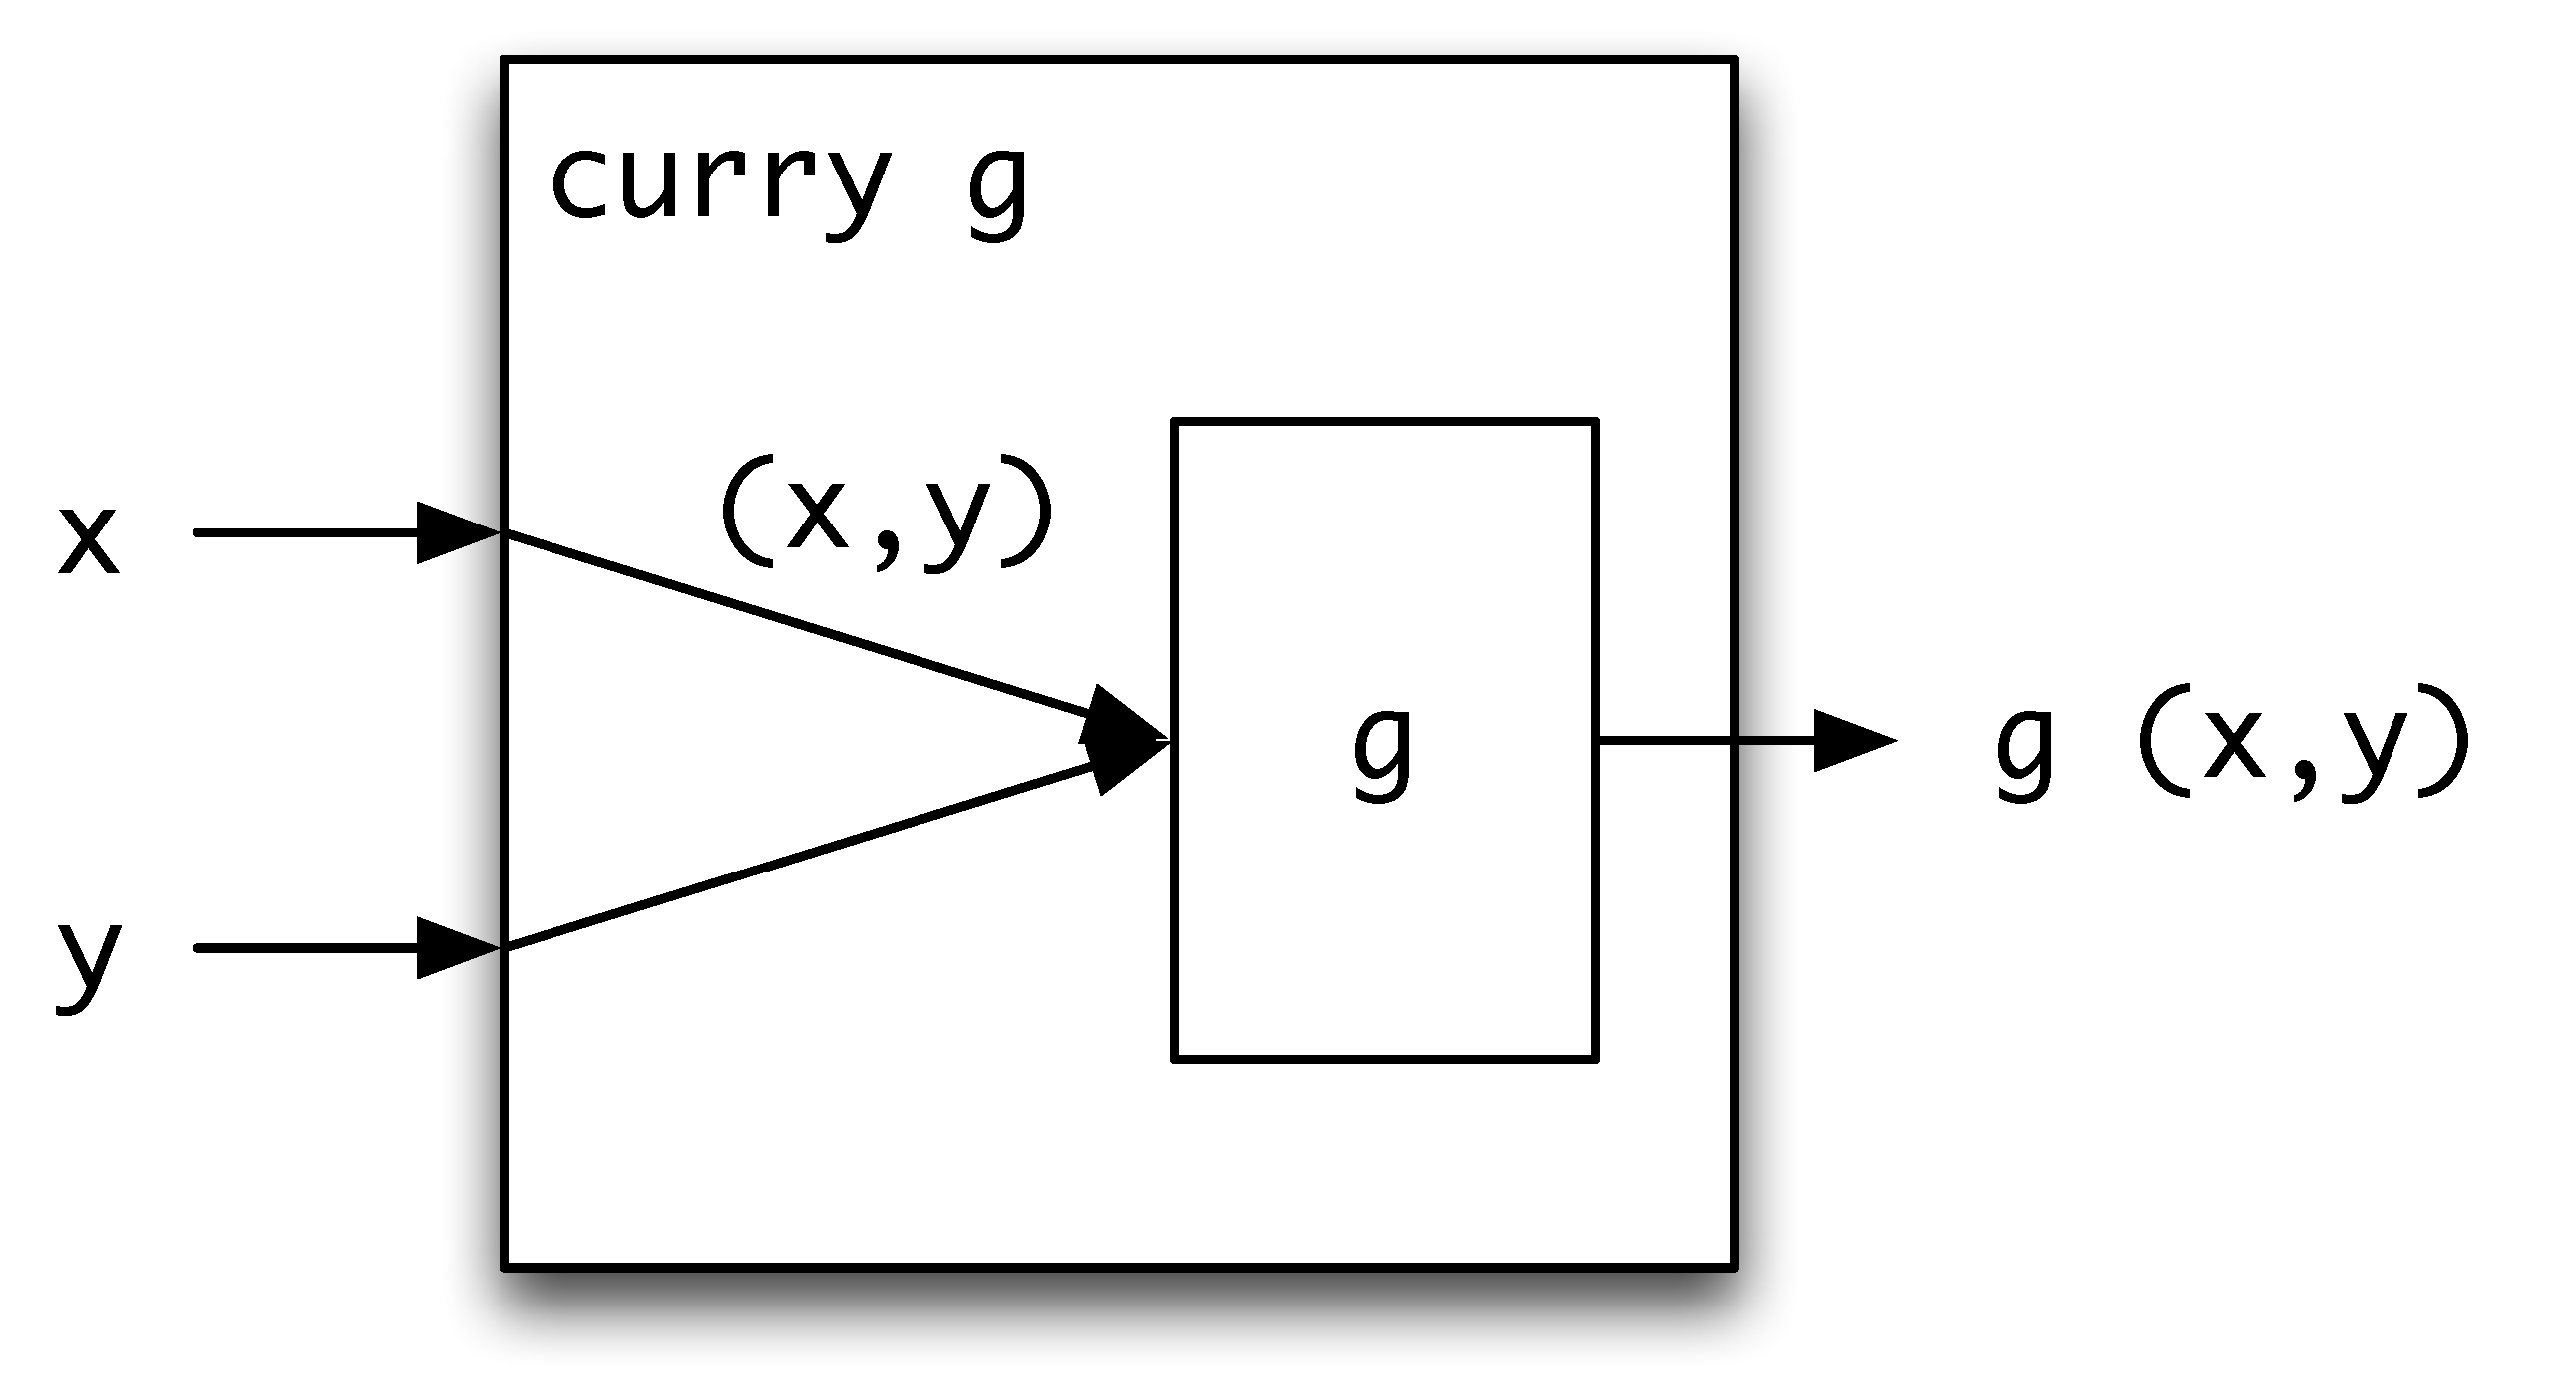
\includegraphics[width=3in]{Pictures/curry.pdf}
\end{center}
This function expects its arguments as a pair, but its curried version,
\texttt{curry g}, will take them separately -- we therefore have to form them into a
pair before applying \texttt{g} to them: 
\begin{alltt}
curry :: ((a,b) -> c) -> (a -> b -> c)\minx{curry}
curry g x y = g (x,y)
\end{alltt}
\texttt{curry multiplyUC} will be exactly the same function as \texttt{multiply}.

Suppose now that \texttt{f} is a curried function, of type 
\texttt{a -> b -> c}. 
\begin{center}
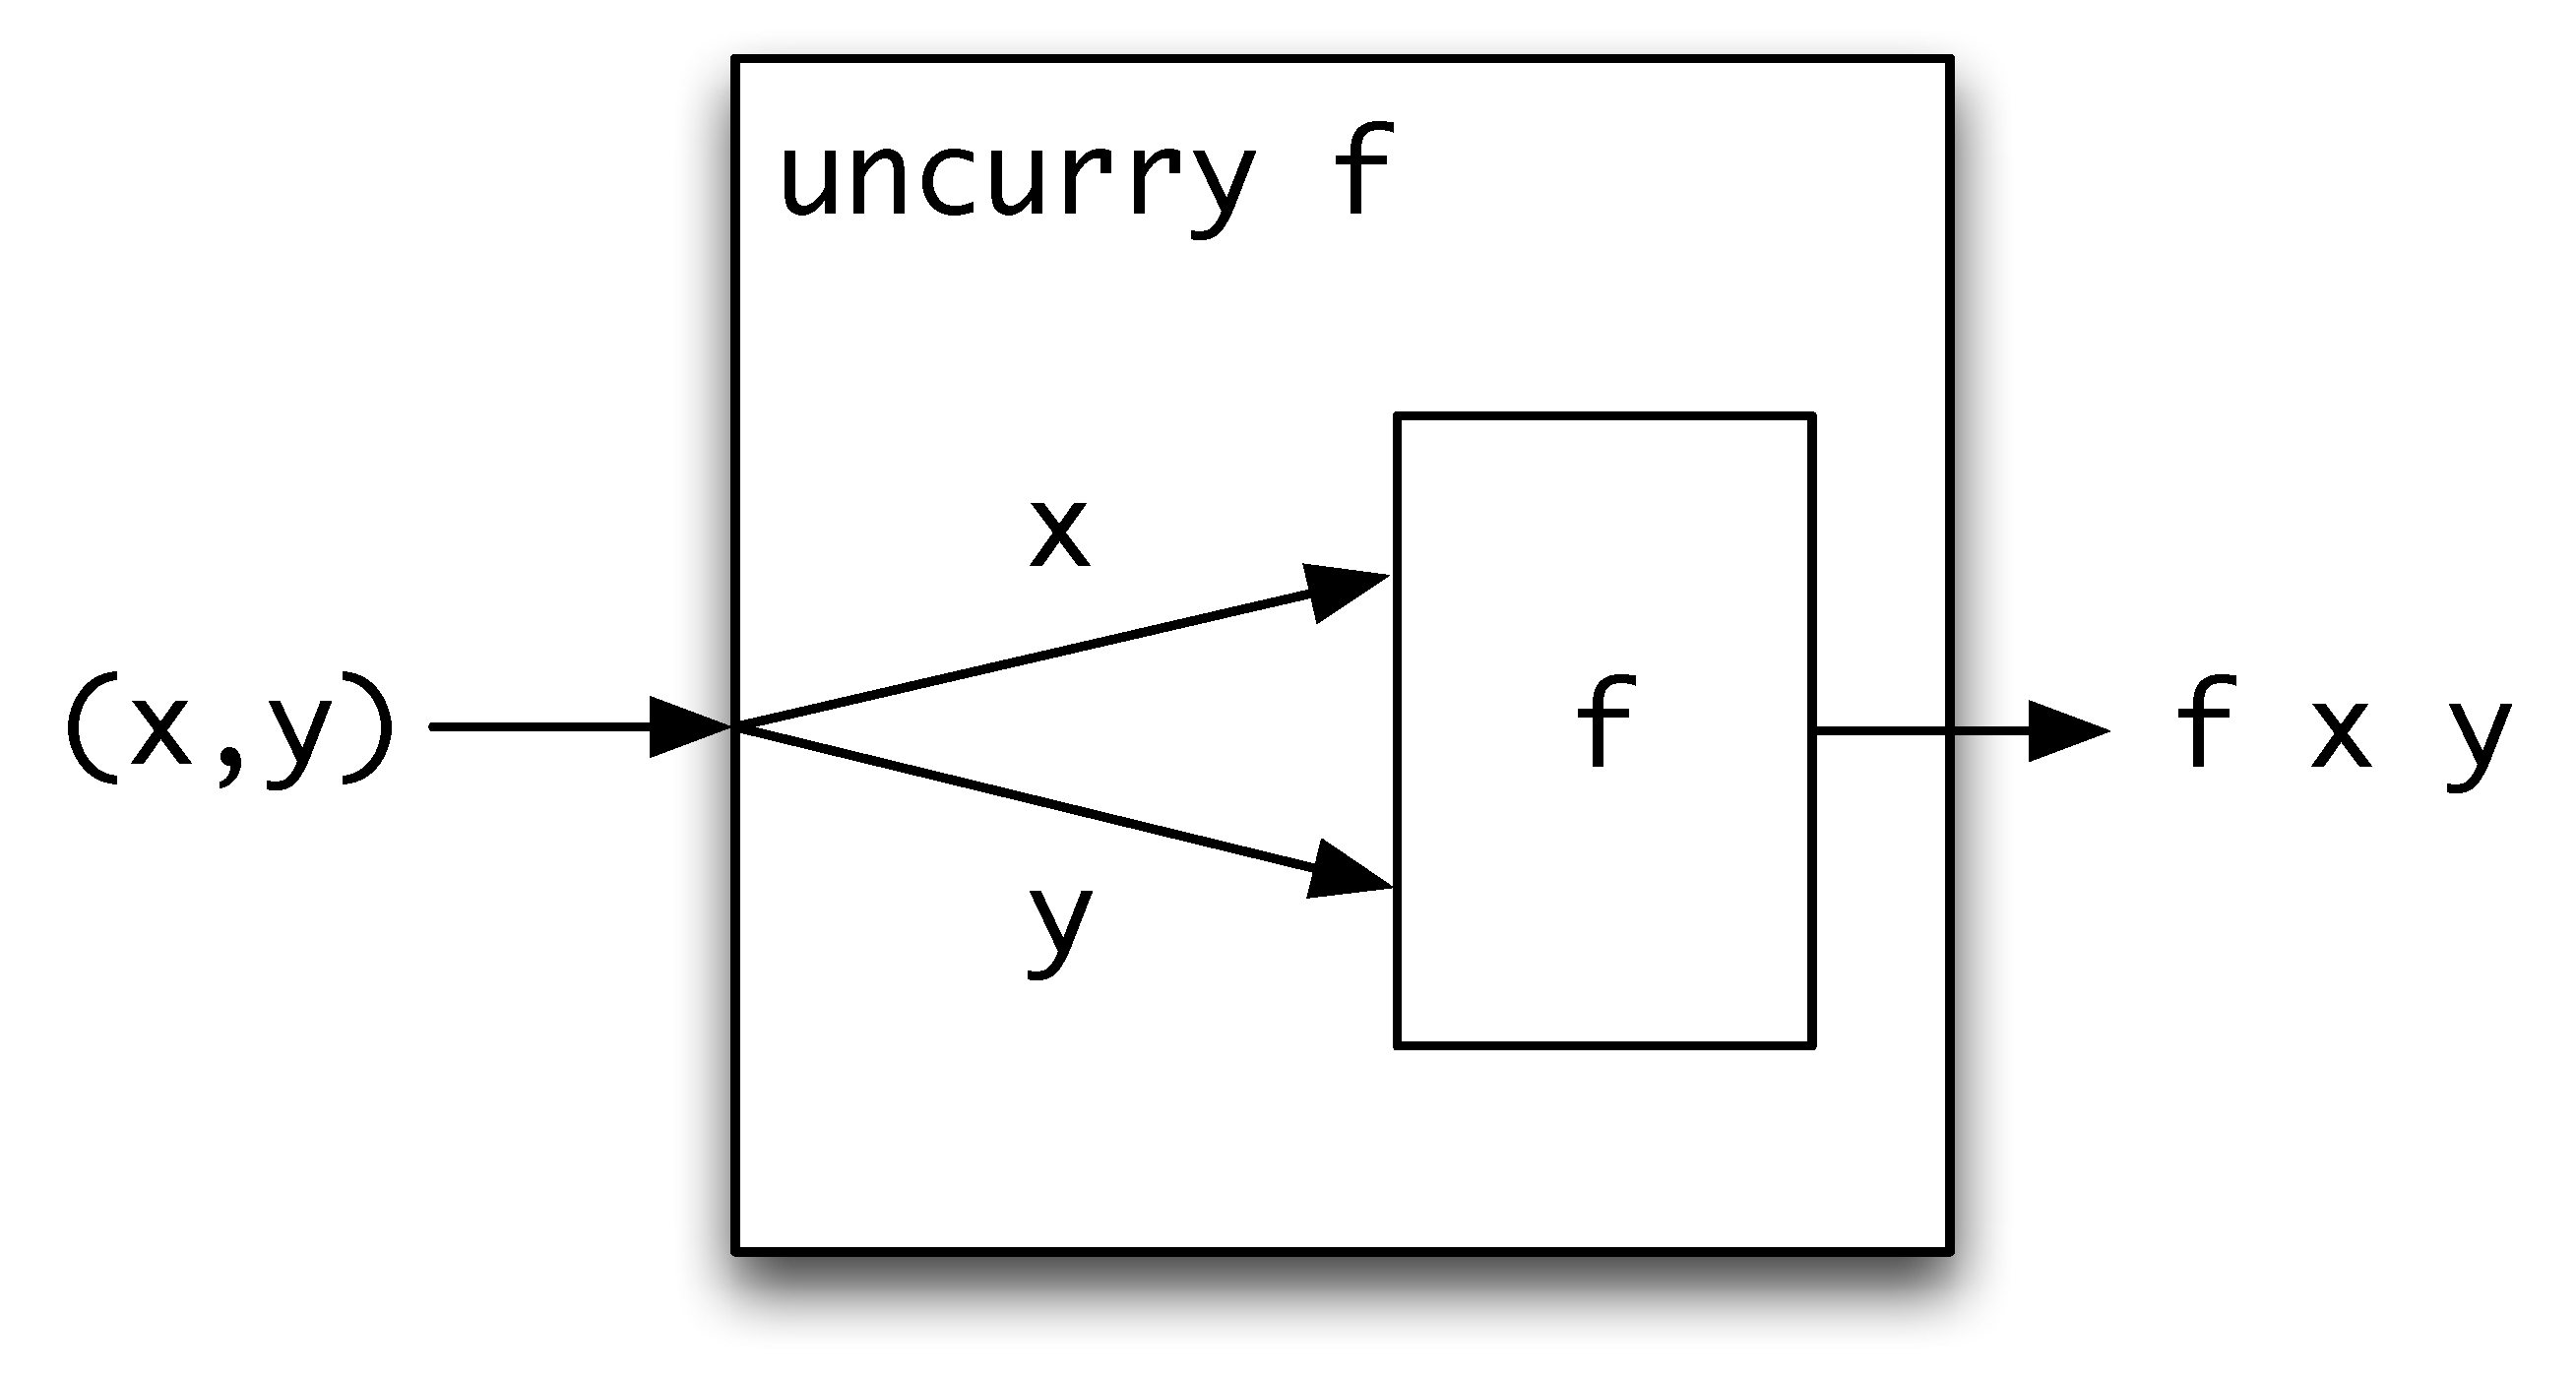
\includegraphics[width=3.0in]{Pictures/uncurry.pdf}
\end{center}
The function \texttt{uncurry f} will expect its
arguments as a pair, and these will have to be separated before
\texttt{f} can be applied to them:
\begin{alltt}
uncurry :: (a -> b -> c) -> ((a,b) -> c)\minx{uncurry}
uncurry f (x,y) = f x y
\end{alltt}
\texttt{uncurry multiply} will be exactly the same function as \texttt{multiplyUC}.
The functions \texttt{curry} and \texttt{uncurry} are inverse to each other.
\index{function!inverse}


A disadvantage of the curried representation of functions is that the inverse of a function like 
\begin{alltt}
unzip ::\ ([a,b]) -> ([a],[b])
\end{alltt}
is not \texttt{zip ::\ [a] -> [b] -> [(a,b)]} but in fact
\begin{alltt}
uncurry zip :: ([a],[b]) -> [(a,b)]
\end{alltt}
(or \texttt{zip'} as we called it earlier in the book) so that statements of properties of these functions, such as
\begin{alltt}
prop_zip xs = uncurry zip (unzip xs) == xs
\end{alltt}
will necessarily involve the uncurried version of the binary function, rather than the curried.

\begin{exercises}

\item
What is the effect of \texttt{uncurry (\$)}? What is its type? Answer a similiar question for \texttt{uncurry (:)}, \texttt{uncurry (.)}.

\item {[Harder]} What are the effects and types of \texttt{uncurry uncurry}, \texttt{curry uncurry}.

\item
Can you state a property relating \texttt{unzip} and \texttt{uncurry zip}, where the latter is the function applied first?

\item
Can you define functions 
\begin{alltt}
curry3 :: ((a,b,c) -> d) -> (a -> b -> c -> d)
uncurry3 :: (a -> b -> c -> d) -> ((a,b,c) -> d)
\end{alltt}
which perform the analogue of \texttt{curry} and \texttt{uncurry} but for three arguments rather than two? Can you use \texttt{curry} and \texttt{uncurry} in these definitions?

\item {[Harder]}
Can you define functions 
\begin{alltt}
curryList :: ([a] -> d) -> (a -> [a] -> d)
uncurryList :: (a -> [a] -> d) -> ([a] -> d)
\end{alltt}
which perform the analogue of \texttt{curry} and \texttt{uncurry} but for a list of  arguments rather than two distinct arguments? Can you use \texttt{curry} and \texttt{uncurry} in these definitions?

\end{exercises}

\index{currying|)}


\section{Defining higher-order functions}
\label{defHOFs}
\index{higher-order function!defining HOFs|(}

This section revises the different ways that we can use to define higher-order functions, and in particular functions that return functions as results. These functions are one of the features of functional programming not shared with most other programming languages that you might be familiar with, and give Haskell particular elegance and power.

\subsection*{Using the operators}

We can use the built-in operators in defining functions directly. We already saw that we could define forward composition in terms of composition,
\begin{alltt}
f >.> g = g.f
\end{alltt}
We also saw this in action in the definition of \texttt{rotate} from the \texttt{Picture} case study:
\begin{alltt}\minx{rotate}
rotate :: Picture -> Picture
rotate = flipV . flipH
\end{alltt}
where again the function is defined directly as the \emph{composition} of two other functions.
The meaning of this definition is just the same as one which has explicit arguments:
\begin{alltt}\minx{rotate}
rotate pic = flipV (flipH pic)
\end{alltt}
but the earlier definition is clearer to read and to
modify; we see \emph{explicitly} that the definition is a composition
of two functions, rather than having to see it as a consequence of the
way the right-hand side is defined in the latter equation.

More importantly, if we state a definition in this form, then we can
apply properties of `\texttt{.}' in analysing how \texttt{rotate}
behaves. This means that in proofs we are able to use properties of composition, as
well as being able to see examples of program transformations which will apply because of the form of composition involved. In general these remarks will apply to all 
higher-order, polymorphic functions, and we see examples of this in Section 
\ref{verifGen} below.


Let's look at some more examples which use composition in their definitions: the 
simplest is this: 
\begin{alltt}
twice f = f.f\hfill (twice.1)\minx{twice}
\end{alltt}
\texttt{f} is a function, and the result is \texttt{f} composed with itself. For
this to work, it needs to have the same input and output type, so we have
\begin{alltt}
twice :: (a -> a) -> (a -> a)
\end{alltt}
This states that \texttt{twice} takes one argument, a function of type 
\texttt{(a -> a)}, and returns a result of the same type. For instance, if \texttt{succ}
is the function to add one to an integer, 
\begin{alltt}
succ :: Integer -> Integer
succ n = n+1
\end{alltt}
then applying \texttt{twice} to it gives the example
\begin{alltt}
(twice succ) 12
\step (succ.succ) 12 \hfill {\rm by} (twice.1)
\step succ (succ 12) \hfill {\rm by definition of } .
\step 14
\end{alltt}
We can generalize \texttt{twice} so that we pass a parameter giving the number
of times the functional argument is to be composed with itself
\begin{alltt}
iter :: Integer -> (a -> a) -> (a -> a)\minx{iter}

iter n f 
  | n>0         = f . iter (n-1) f\hfill(iter.1)
  | otherwise   = id\hfill(iter.2)
\end{alltt}
This is a standard primitive recursion over the integer argument; in the
positive case we take the composition of \texttt{f} with itself
\texttt{n-1} times and compose once more with \texttt{f}. In the zero case
we apply \texttt{f} no times, so the result is a function which returns its argument unchanged, namely \texttt{id}. 

As an example of using \texttt{iter}, we can define \texttt{\superscr{2}{n}} as \texttt{iter n double
1}, if \texttt{double} doubles its argument. 


\begin{exercises}

\item
Give calculations of
\begin{alltt}
{\hskip1pc}iter 3 double 1
(comp2 succ (*)) 3 4
comp2 sq add 3 4
\end{alltt}

\item
What is the type and effect of the function
\begin{alltt}
\bs{n} -> iter n succ
\end{alltt}

\item 
Give an alternative ``constructive'' definition of \texttt{iter} which creates the list of \texttt{n} copies of \texttt{f}
\begin{alltt}
[f,f,...,f]
\end{alltt} and then composes these functions by folding in the
operator `\texttt{.}' to give 
\begin{alltt}
f . f . \ldots\ . f
\end{alltt}



\end{exercises}

\subsection*{Using local definitions}

Local definitions allow us to define functions as a subsidiary part of a function definition. We looked earlier at the example of 
\begin{alltt}
addNum :: Integer -> Integer -> Integer
\end{alltt}
We can use a local definition to give the result, either using a \texttt{where}
\begin{alltt}
addNum n = addN
		   where
		   addN m = n+m
\end{alltt}
or a \texttt{let}
\begin{alltt}
addNum n = let 
             addN m = n+m
           in
             addN
\end{alltt}
This gives us a way of defining results which are functions by locally defining that function and returning it as the result; it has the advantage of not requiring any more advanced machinery, but the disadvantage of introducing a named definition of \texttt{addN} which is extraneous to the actual result. 		   

\subsection*{Lambda abstractions}

Let's try to define a function that takes a binary function as argument, and which returns a binary function that takes its arguments in the opposite order; let's call it \texttt{flip}:
\begin{alltt}
flip :: (a -> b -> c) -> (b -> a -> c)\minx{flip}
\end{alltt}
We can use a lambda abstraction to give the result:
\begin{alltt}
flip f = \bs{}x y -> f y x\hfill(flip.1)
\end{alltt}
This makes clear that a function like
\texttt{flip map} takes as its first argument the list and as its second
the function to be mapped; it can then be partially applied to its first argument, having
the effect of applying \texttt{map} to its second only. This allows us to do a partial application to the second argument of a two argument function.

\subsection*{Partial application}

Partial applications give us a particularly direct way of defining some higher order functions. Taking the example we have just looked at, we can instead say
\begin{alltt}\minx{flip}
flip f x y = f y x
\end{alltt}
If we apply \texttt{flip} to one argument, we have a function which behaves just as described in \texttt{(flip.1)}. Similarly, the behaviour of 
\begin{alltt}
addNum n = addN
		   where
		   addN m = n+m
\end{alltt}
is given by the simple definition
\begin{alltt}
addNum n m = n+m
\end{alltt}
partially applied to \texttt{n}.

\beware{Constructors are functions too}{
Datatype constructors are functions, and so they can be partially applied, passed as arguments to functions or indeed returned as results. To give just one example, this expression creates a list of \texttt{People} from lists of names and ages:
\begin{alltt}
zipWith Person ["Geraint","Bob"] [45,67]
\end{alltt}
}

\begin{figure}[t]\index{point-free programming}
\beware{Point-free programming}{
Some function-level, or `point-free', definitions express what the function does with real clarity: writing\label{pointfree}
\texttt{
flipV = map reverse\ }
precisely describes how to flip a picture in a vertical mirror. However, it is possible to take this approach too far, and write definitions which it's very hard to understood. For instance, what does this function do:
\begin{alltt}
puzzle = (.) (.)
\end{alltt}
Reading the definition tells us that it is the composition operator partially applied to itself, but still it's not clear what the function will do. How can we work out what it does? The best way is to apply it to some arguments and see what it does:
\begin{alltt}
(.) (.) x \step{}(.).x
\end{alltt}
so
\begin{alltt}
(.) (.) x y \step{}((.).x) y \step{}(.) (x y)
\end{alltt}
Applying to a third argument gives
\begin{alltt}
(.) (.) x y z \step \ldots\ \step{}(.) (x y) z \step{}(x y) . z
\end{alltt}
and finally 
\begin{alltt}
(.) (.) x y z w \step \ldots\ \step{}((x y) . z) w \step{}(x y) (z w)
\end{alltt}
giving us the much more informative explanation:
\begin{alltt}
puzzle x y z w = (x y) (z w)
\end{alltt}
Finally, we use to get GHCi to give its type, like this \texttt{:type (.)(.)} and get
\begin{alltt}
(.)(.) :: (a1 -> b -> c) -> a1 -> (a -> b) -> a -> c
\end{alltt}
So there we are \ldots\ To be fair, once we understand what \texttt{puzzle} does, it can be useful to have the original definition which explicitly uses the composition operator, because then any general laws that we discover for \texttt{(.)} will apply to \texttt{puzzle} too.
}
\end{figure}




\subsection*{Examples}

We conclude this section by exploring how partial applications and operator sections can be
used to simplify and shorten definitions in a number of other examples. 
Often it is possible to avoid
giving an explicit function definition if we can use a partial application to
return a function. Revisiting the examples of Chapter \ref{defFunLists} we see that
to double all the elements in a list we can write
\begin{alltt}
doubleAll :: [Int] -> [Int]
doubleAll = map (*2)\minx{doubleAll}
\end{alltt}
using an operator section \texttt{(*2)} to replace the \texttt{double} function,
and giving the function definition directly by partially applying \texttt{map}.

To filter out the even elements in a numerical list, we have to check whether
the remainder on dividing by two is equal to zero. As a function we can write
\begin{alltt}
(==0).(`mod` 2)
\end{alltt}
This is the composition of two operator sections: first find the remainder on dividing by
two,
then check if it is equal to zero. (Why can we not write \texttt{(`mod` 2 ==
0)}?) The filtering function can then be written
\begin{alltt}\minx{getEvens}
getEvens :: [Int] -> [Int]
getEvens = filter ((==0).(`mod` 2))
\end{alltt}
Our final example comes from the list splitting study. We defined
\begin{alltt}
getWord xs 
  = getUntil p xs\minx{getWord}
    where 
    p x = elem x whitespace
\end{alltt}
The local definition is not now needed, as we can define the function \texttt{p}
by an operator section:
\begin{alltt}\minx{getWord}
getWord xs = getUntil (`elem` whitespace) xs
\end{alltt}
Note the way that we partially apply a
function to its {\em second\/} argument, by forming an operator section. This
works because
\begin{alltt}
(`elem` whitespace) x
= x `elem` whitespace
= elem x whitespace
\end{alltt}
as required.

Finally, the 
function \texttt{getWord} can itself be given a direct definition,
by partial application thus
\begin{alltt}
getWord = getUntil (`elem` whitespace)
\end{alltt}
This definition reads like an informal explanation -- to get a word, get
characters until a whitespace character is found.
 


\begin{exercises}

\item
Using partial application re-define the function 
\begin{alltt}
mapFuns :: [a->b] -> a -> [b]
\end{alltt}
first defined in Section \ref{exprFuns}.


\item
{[Harder]} Define a function
\begin{alltt}
{\hskip1pc}slope :: (Float -> Float) -> (Float -> Float)
\end{alltt}
which takes a function \texttt{f} as argument, and returns (an approximation to)
its derivative \texttt{f'} as result.


\item
{[Harder]} Define a function
\begin{alltt}
{\hskip1pc}integrate :: (Float -> Float) -> (Float -> Float -> Float)
\end{alltt}
which takes a function \texttt{f} as argument, and returns (an approximation to)
the two argument function which gives the area under its graph between two end
points as its result.

\end{exercises}
  
\index{higher-order function!defining HOFs|)}




\markright{Verification and general functions}

\section[Verification and general functions]{Verification and
general functions}
\index{proof!higher-order functions|(}
\index{higher-order function!proofs}
\label{verifGen}
\markright{Verification and general functions}

Verification can take on a different character when we look at higher-order
polymorphic functions. We can start to prove equalities between functions,
rather than between values of functions, and we shall also see that we are able
to prove theorems which resemble their subjects in being general and reusable,
and so applicable in many contexts.

\subsection*{Function-level verification}
\index{proof!function level}

We claimed in Section \ref{defHOFs} that the function \texttt{iter} is
a generalization of \texttt{twice}, since
\begin{alltt}\minx{iter}\minx{twice}
iter 2 f
  = f . iter 1 f\hfill {\rm by} (iter.1)
  = f . (f . iter 0 f)\hfill {\rm by} (iter.1)
  = f . (f . id)\hfill {\rm by} (iter.2)
  = f . f\hfill {\rm by} (compId)
  = twice f\hfill {\rm by} (twice.1)
\end{alltt}
In proving this we have used the equality between two functions
\begin{alltt}
f . id = f \hfill \texttt{(compId)}
\end{alltt}
How is this proved? We examine how each side behaves on an arbitrary argument
\texttt{x}
\begin{alltt}
(f . id) x
  = f (id x)
  = f x
\end{alltt}
so that for any argument \texttt{x} the two functions have the same
behaviour. As black boxes, they are therefore the same. 
As what interests us here is their behaviour,
we say that they are equal. We call this `black-box' concept of equality 
\textbf{extensional}.

\begin{definition}{{\sffamily Principle of extensionality:}
\index{extensionality principle}
\medskip

\noindent
Two functions \texttt{f} and \texttt{g} are equal if they have the same value at
every argument.}
\end{definition}

\noindent
This is called extensionality in contrast to the idea of\index{intensionality} 
\textbf{intensionality} in which we say two functions are the same only if they have
the same definitions -- we no longer think of them as black boxes; we
are allowed to look inside them to see how the mechanisms work, as it were. If
we are interested in the results of our programs, all that matters are the
values given by functions, not how they are arrived at. We therefore use
extensionality when we are reasoning about function behaviour in Haskell. If
we are interested in \textbf{efficiency} or other performance aspects of
programs, then the way in which a result is found {\em will\/} be significant,
however. This is discussed further in Chapter \ref{behaviour}.

\begin{exercises}


\item
Using the principle of extensionality, show that function composition 
is associative: that is, for all \texttt{f}, {\mi
g} and \texttt{h},
\begin{alltt}
f . (g . h) = (f . g) . h
\end{alltt}\index{function composition!associative}

\item
Show that for all \texttt{f},
\begin{alltt}
id . f = f
\end{alltt}

\item
Show that the function \texttt{flip} defined in Section \ref{curry} satisfies
\begin{alltt}
flip . flip = id
\end{alltt}
Hint: to show this, you might want to prove that for any \texttt{f},
\begin{alltt}
flip (flip f) = f
\end{alltt}

\item
Two functions \texttt{f} and \texttt{g} are \textbf{inverses} if it can be shown that
\index{function!inverse}
\begin{alltt}
f . g = id              g . f = id
\end{alltt}
Prove that the functions \texttt{curry} and \texttt{uncurry} of Section \ref{curry}
are inverses. Can you think of other pairs of inverse functions?

\item
Using induction, prove that for all natural numbers \texttt{n},
\begin{alltt}
iter n id = id
\end{alltt}

\item
A function \texttt{f} is called \textbf{idempotent} if\index{idempotence} 
\begin{alltt}
f . f = f
\end{alltt}
Show that the functions \texttt{abs} and \texttt{signum} are idempotent. Can you
think of any other idempotent functions?
\end{exercises}

\subsection*{Higher-level proofs}
\index{proof!higher-level}

Our verification thus far has concentrated on first-order, monomorphic
functions. Just as \texttt{map}, \texttt{filter} and \texttt{fold} generalize
patterns of definition, we shall find that proofs about these functions
generalize results we have seen already. To give some examples, it is
not hard to prove that
\begin{alltt}
doubleAll (xs++ys) = doubleAll xs ++ doubleAll ys\minx{doubleAll}
\end{alltt}
holds for all finite lists \texttt{xs} and \texttt{ys}.
When \texttt{doubleAll} is defined as \texttt{map (*2)} it becomes clear that we have an
example of a general result,
\begin{alltt}\index{map@\texttt{map}}
map f (xs++ys) = map f xs ++ map f ys\index{map@\texttt{map}}\hfill(map++)
\end{alltt}
which is valid for {\em any\/} function \texttt{f}.
We also claimed in an earlier exercise that
\begin{alltt}
sum (xs++ys) = sum xs + sum ys\hfill (sum.3)
\end{alltt}
for all finite lists \texttt{xs}, \texttt{ys}. The function \texttt{sum} is given by
folding in \texttt{(+)}, 
\begin{alltt}\minx{sum}\index{foldr@\texttt{foldr}}
sum = foldr (+) 0
\end{alltt}
and we have, generally,
if \texttt{f} is associative, and \texttt{st} is an identity for \texttt{f}, that is,
\begin{alltt}\label{assocId}
x `f` (y `f` z) = (x `f` y) `f` z
x `f` st = x = st `f` x
\end{alltt}
for all \texttt{x}, \texttt{y}, \texttt{z}
then the equation 
\begin{alltt}
foldr f st (xs++ys) = f (foldr f st xs) (foldr f st ys)\hfill (foldr.3)\index{foldr@\texttt{foldr}}
\end{alltt}
holds for all finite \texttt{xs} and \texttt{ys}. Obviously \texttt{(+)} is associative and has
\texttt{0} as an identity, and so \texttt{(sum.3)} is a special case of
\texttt{(foldr.3)}.
Now we give three proofs of examples in the same vein.

\subsection*{\texttt{map} and composition}
\index{function composition}\index{map@\texttt{map}}

A first example concerns \texttt{map} and composition. Recall the definitions
\begin{alltt}
map f []     = [] \hfill (map.1)
map f (x:xs) = f x : map f xs\hfill (map.2)
(f . g) x    = f (g x)\hfill (comp.1)
\end{alltt}
It is not hard to see that we should be able to prove that
\begin{alltt}
map (f . g) xs = (map f . map g) xs \hfill (map.3)
\end{alltt}
holds for every
finite list \texttt{xs}. 
\begin{center}
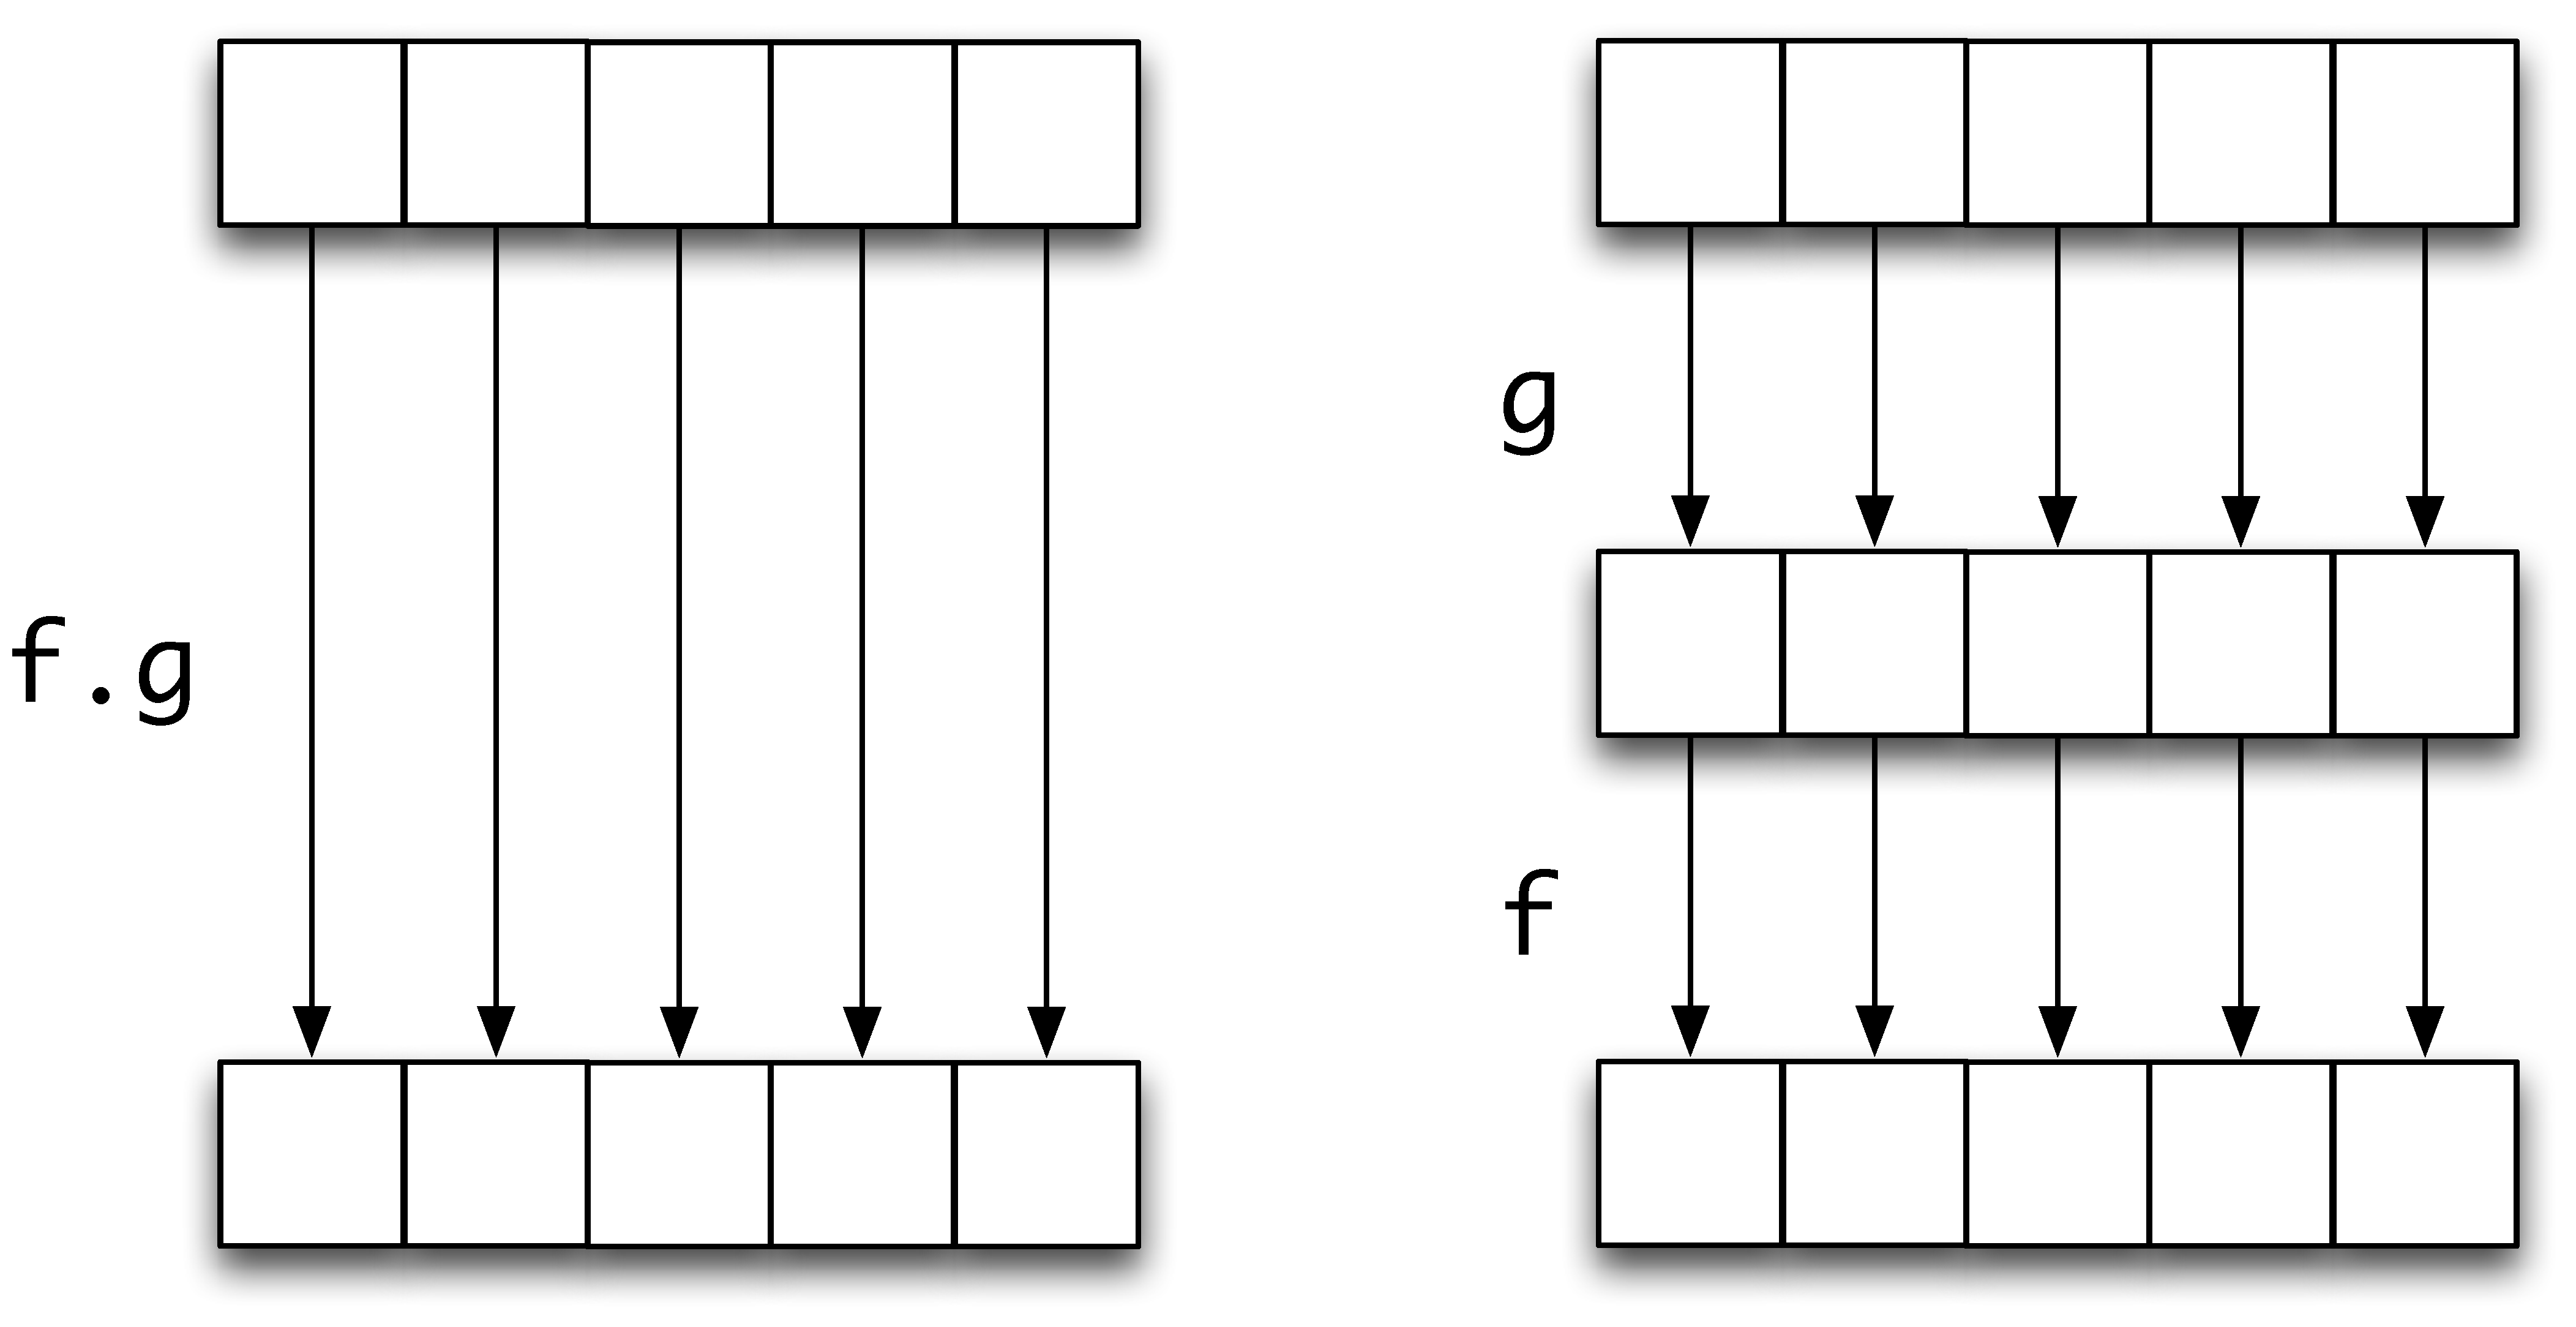
\includegraphics[width=3.5in]{Pictures/mapComp.pdf}
\end{center}
Applying 
\texttt{(f .\ g)} to every member of a list should be the same as applying \texttt{g} to
every member of the list and then applying \texttt{f} to every member of the result. It is proved
just as easily, by structural induction\index{structural induction}. 
The \texttt{(base)} case requires the identity
to be proved for the empty list.
\begin{alltt}
map (f . g) [] = [] \hfill {\rm by} (map.1)
\bl
(map f . map g) [] 
  = map f (map g []) \hfill {\rm by} (comp.1)
  = map f [] \hfill {\rm by} (map.1)
  = [] \hfill {\rm by} (map.1)
\end{alltt}
Assuming that 
\begin{alltt}
map (f .\ g) xs = (map f .\ map g) xs\hfill(hyp)
\end{alltt} is true,
it is now necessary to prove that 
\begin{alltt}
map (f . g) (x:xs) = (map f . map g) (x:xs)\hfill(ind)
\end{alltt}
Again, it is enough to analyse each side of the equation.
\begin{alltt}
map (f . g) (x:xs) 
  = (f . g) x : map (f . g) xs \hfill {\rm by} (map.2)
  = f (g x) : map (f . g) xs \hfill {\rm by} (comp.1)
\bl
(map f . map g) (x:xs) 
  = map f (map g (x:xs)) \hfill {\rm by} (comp.1)
  = map f (g x : map g xs) \hfill {\rm by} (map.2)
  = f (g x) : map f (map g xs) \hfill {\rm by} (map.2)
  = f (g x) : (map f . map g) xs \hfill {\rm by} (comp.1)
\end{alltt}
The induction hypothesis is exactly what is needed to prove the two sides
equal,
completing the proof of the induction step and the proof itself. \blackbox

Each Haskell list type, besides containing finite lists,
also contains infinite and partial lists. In Chapter \ref{lazy}
these will be explained and it will be shown that 
\texttt{(map.3)} is true for {\em all\/} lists \texttt{xs}, and therefore that the functional
equation
\begin{alltt}
map (f . g) = (map f) . (map g)
\end{alltt}
holds in general.

\subsection*{\texttt{map} and \texttt{filter}}
\index{map@\texttt{map}}\index{filter@\texttt{filter}}


The proof above showed how properties of functional programs could be proved
from the definitions of the functions in a straightforward way. The properties
can state how the program behaves -- that a sorting function returns an ordered
list, for instance -- or can relate one program to another. This latter idea
underlies \textbf{program transformation}\index{program transformation}
for functional languages. This section
introduces an example 
called \textbf{filter promotion} which is one of the most
useful of the basic functional transformations.
\begin{alltt}
filter p . map f = map f . filter (p . f)\hfill(filter/map)\label{filterMap}
\end{alltt}
The equation says that a \texttt{map} followed by a \texttt{filter} can be replaced
by a \texttt{filter} followed by a \texttt{map}. The right-hand side is potentially
more efficient than the left, since the \texttt{map} operation will there be
applied to a shorter list, consisting of just those elements with the property
\texttt{(p .\ f)}.
An example is given by the function first defined in Section \ref{opsecs}.
\begin{alltt}
filter (0<) . map (+1)
\end{alltt}
Instead of mapping first, the function can be replaced by
\begin{alltt}
map (+1) . filter ((0<) . (+1))
 = map (+1) . filter (0<=)
\end{alltt}
and it is clear that here the transformed version is more efficient,
since the test \texttt{(0<=)} is no more
costly than \texttt{(0<)}.
The proof that
\begin{alltt}
(filter p . map f) xs = (map f . filter (p . f)) xs
\end{alltt}
for finite lists \texttt{xs} is by structural induction.\index{structural
induction}
First we reiterate the definitions of \texttt{map}, \texttt{filter} and {\mi
composition}.
\begin{alltt}
map f []        = [] \hfill (map.1)
map f (x:xs)    = f x : map f xs\hfill (map.2)
\bl
filter p []     = []\hfill (filter.1)
filter p (x:xs) 
  | p x         = x : filter p xs\hfill (filter.2)
  | otherwise   =     filter p xs\hfill (filter.3)
\bl
(f . g) x       = f (g x)\hfill (comp.1)
\end{alltt}
The base case consists of a proof of 
\begin{alltt}
(filter p . map f) [] = (map f . filter (p . f)) [] \hfill (base)
\end{alltt}
This is true since
\begin{alltt}
(filter p . map f) []
  = filter p (map f []) \hfill {\rm by} (comp.1)
  = filter p [] \hfill {\rm by} (map.1)
  = [] \hfill {\rm by} (filter.1)
\end{alltt}
and
\begin{alltt}
(map f . filter (p . f)) []
  = map f (filter (p . f) [])  \hfill {\rm by} (comp.1)
  = map f []  \hfill {\rm by} (filter.1)
  = []  \hfill {\rm by} (map.1)
\end{alltt}
In the induction step, a proof of 
\begin{alltt}
(filter p . map f) (x:xs) = (map f . filter (p . f)) (x:xs) \hfill (ind)
\end{alltt}
is required, using the induction hypothesis
\begin{alltt}
(filter p . map f) xs = (map f . filter (p . f)) xs \hfill (hyp)
\end{alltt}
The proof begins with an analysis of the left-hand side of \texttt{(ind)}.
\begin{alltt}
(filter p . map f) (x:xs)
  = filter p (map f (x:xs))  \hfill {\rm by} (comp.1)
  = filter p (f x : map f xs) \hfill {\rm by} (map.2)
\end{alltt}
There are two\footnote{
We should also think about what happens when {\smtt p (f x)} is undefined; in
this case both sides will be undefined, and so equal.}
cases\index{proof!by cases} to consider:
whether \texttt{p (f x)} is \texttt{True} or \texttt{False}. Taking the case
where  \texttt{p (f x)} is \texttt{True}, we continue to examine the left-hand
side of \texttt{(ind)}, giving
\begin{alltt}
  = f x : filter p (map f xs)  \hfill {\rm by} (filter.2)
  = f x : (filter p . map f) xs \hfill {\rm by} (comp.1)
  = f x : (map f . filter (p . f)) xs \hfill {\rm by} (hyp)
\end{alltt}
Now we look at the right-hand side of \texttt{(ind)}, also assuming 
that \texttt{p (f x)} is \texttt{True}:
\begin{alltt}
(map f . filter (p . f)) (x:xs) 
  = map f (filter (p . f) (x:xs))\hfill {\rm by} (comp.1) 
  = map f (x: (filter (p . f) xs))\hfill {\rm by} (filter.2) 
  = f x : map f (filter (p . f) xs)\hfill {\rm by} (map.2)
  = f x : (map f . filter (p . f)) xs \hfill {\rm by} (comp.1)
\end{alltt}
which shows that \texttt{(ind)} holds in the case that \texttt{p (f
x)} is \texttt{True}.

A similar chain of reasoning gives the same result in the case where
\texttt{p (f x)} is \texttt{False}. This establishes \texttt{(ind)} assuming \texttt{(hyp)}, and so
together with \texttt{(base)} completes the proof of the filter promotion
transformation in the case of finite lists; it holds, in fact, for all
lists. \blackbox

\begin{figure}[t]\index{QuickCheck!and higher-order functions}\index{higher-order function!QuickCheck}
\beware{QuickCheck and higher-order functions}
{\label{QChofs}We've already seen that QuickCheck is a very good way of checking whether particular properties hold for functions that we define. QuickCheck works by generating random test  data and checking whether properties hold at these values. While generating data is not entirely straightforward for structured types like lists and algebraic types, it can be done. Generating random functions is more difficult, and isn't supported ``out of the box'' by QuickCheck: for it to work we need to be able to ``show'' functions. We examine how to do this, and so how to use QuickCheck to test properties involving higher-order functions, in Chapter \ref{dsls}. In the meantime we look at how to check properties for given functions and randomly-generated lists.

\medskip
Let's take the example of the property for \texttt{map} and \texttt{filter}, \texttt{(filter/map)} introduced on page \pageref{filterMap}:
\begin{alltt}
prop_mf p f = 

\ \ \ \ \bs{}xs -> (filter p . map f) xs == (map f . filter (p . f)) xs
\end{alltt}
We can check this for specific values of \texttt{p} and \texttt{f} like this
\begin{alltt}
\textsl{Prompt>} quickCheck (prop_mf (>0) (\bs{}x -> x*x))

\textsl{+++ OK, passed 100 tests.}

\textsl{Prompt>} quickCheck (prop_mf (>=0) (\bs{}x -> x*x*x))

\textsl{+++ OK, passed 100 tests.}
\end{alltt}
where for each instance of \texttt{p} and \texttt{f} the property is tested for 100 randomly generated values.
}\end{figure}


\subsection*{\texttt{map}, \texttt{reverse} and the \texttt{Picture} case study}
\index{map@\texttt{map}}\minx{reverse}\index{pictures}

When we introduced the \texttt{Picture} case study
in Chapter \ref{intro} we claimed that we could prove that 
\texttt{flipV} and \texttt{flipH}
can be applied in either order to give the same result. Our
implementation defines them thus
\begin{alltt}\minx{flipH}\minx{flipV}
flipH = reverse
flipV = map reverse
\end{alltt}
and we can see informally that 
\begin{itemize}
\item
\texttt{reverse} affects the order of the elements, while leaving the
elements unchanged;
\item 
\texttt{map reverse} affects each of the elements, while keeping their
order the same.
\end{itemize}
The second observation is a consequence of the function being a
\texttt{map}, and so we make the more general claim that for all finite lists \texttt{xs} and all
functions \texttt{f},
\begin{alltt}
map f (reverse xs) = reverse (map f xs)\hfill(map/reverse)
\end{alltt}
This has the consequence that
\begin{alltt}
flipV (flipH xs) = flipH (flipV xs)
\end{alltt}
if we replace \texttt{f} in \texttt{(map/reverse)}
by \texttt{reverse}. We will see in Chapter \ref{lazy} that we can
establish
\texttt{(map/reverse)}
for all lists \texttt{xs} and so conclude that the functional equations
hold:
\begin{alltt}
map f . reverse = reverse . map f
flipV . flipH   = flipH . flipV
\end{alltt}
We now prove \texttt{(map/reverse)}
by induction over \texttt{xs}.

We have seen the definition of \texttt{map} in the previous examples;
\texttt{reverse} is defined thus.
\begin{alltt}
reverse []     = []\hfill(reverse.1)
reverse (z:zs) = reverse zs ++ [z]\hfill(reverse.2)
\end{alltt}

\subparagraph{Statement} We first have to prove the base case:
\begin{alltt}
map f (reverse []) = reverse (map f [])\hfill(base)
\end{alltt}
and then we need to prove the induction step,
\begin{alltt}
map f (reverse (x:xs)) = reverse (map f (x:xs))\hfill(ind)
\end{alltt}
assuming the induction hypothesis:
\begin{alltt}
map f (reverse xs) = reverse (map f xs)\hfill(hyp)
\end{alltt}

\subparagraph{Base} Looking at the two sides of the base case in turn, we
have
\begin{alltt}
map f (reverse [])
  = map f [] \hfill {\rm by} (reverse.1)
  = [] \hfill {\rm by} (map.1)

reverse (map f [])
  = reverse [] \hfill {\rm by} (map.1)
  = [] \hfill {\rm by} (reverse.1)
\end{alltt}
and this shows that the two sides of the base case equation have the same value, and so
we move on to the induction case.

\subparagraph{Induction} 
We start by examining the left-hand side of \texttt{(ind)}:
\begin{alltt}
map f (reverse (x:xs)) 
  = map f (reverse xs ++ [x])\hfill {\rm by} (reverse.2)
\end{alltt}
Now, it is not hard to prove that
\begin{alltt}
map f (ys++zs) = map f ys ++ map f zs\hfill (map++)
\end{alltt}
(we leave this proof as an exercise for the reader)
and using \texttt{(map++)} we can continue to simplify the left-hand side
\begin{alltt}
  = map f (reverse xs) ++ map f [x] \hfill {\rm by} (map++)
  = map f (reverse xs) ++ [f x]  \hfill {\rm by} (map.1),(map.2)
\end{alltt}
Using the induction hypothesis, we can make one more step,
\begin{alltt}
  = reverse (map f xs) ++ [f x]\hfill {\rm by} (hyp)
\end{alltt}
Now looking at the right-hand side,
\begin{alltt}
reverse (map f (x:xs))
  = reverse (f x : map f xs) \hfill {\rm by} (map.2)
  = reverse (map f xs) ++ [f x]\hfill {\rm by} (reverse.2) 
\end{alltt}
and now we see that the two sides are equal, which establishes the
induction step and so completes the proof. \blackbox
\index{proof!higher-order functions|)}

\subsection*{Libraries of theorems}
\index{proof!libraries of theorems}

We have seen in this section that we can prove properties of general
functions like \texttt{map}, \texttt{filter}
and \texttt{foldr}. This means that when we define a function which
uses \texttt{map}, say, we can call on a whole library of properties of
\texttt{map}, including, for all finite \texttt{xs} and \texttt{ys}:
\begin{alltt}
map (f . g) xs        = (map f . map g) xs
(filter p . map f) xs = (map f . filter (p . f)) xs
map f (reverse xs)    = reverse (map f xs)
map f (ys++zs)        = map f ys ++ map f zs
\end{alltt}
We have seen that
 using the general functions \texttt{map}, \texttt{filter} and others allowed us to
make direct definitions of new functions rather than having to define them `from scratch'
using recursion. In exactly the same way,
these general theorems will mean that in many cases we can avoid writing an
induction proof about our specific function, and instead simply use one of these theorems.  


\begin{exercises}


\item 
Prove that for all \texttt{ys} and \texttt{zs} the equation
\begin{alltt}
map f (ys++zs) = map f ys ++ map f zs\hfill (map++)
\end{alltt}
as was used in the proof of the theorem about \texttt{map} and
\texttt{reverse}.


\item
If \texttt{f} is associative, and \texttt{st} is an identity for {\mi
f} -- these notions were defined on page \pageref{assocId} -- then prove that
the equation \texttt{(foldr.3)}:
\begin{alltt}
foldr f st (xs++ys) = f (foldr f st xs) (foldr f st ys)
\end{alltt}
holds for all
finite \texttt{xs} and \texttt{ys}.

\item
Argue that the result
\begin{alltt}
concat (xs ++ ys) = concat xs ++ concat ys
\end{alltt} 
is a special case of \texttt{(foldr.3)},  using 
\begin{alltt}
concat = foldr (++) []
\end{alltt}
as the definition of \texttt{concat}.

\item
Prove that for all finite lists \texttt{xs}, and functions \texttt{f},
\begin{alltt}
concat (map (map f) xs) = map f (concat xs)
\end{alltt}

\item
Prove that over the type \texttt{Int}
\begin{alltt}
(0<) . (+1) = (0<=)
\end{alltt}
as is used in the theorem relating \texttt{map} and \texttt{filter}.

\item
Prove for all finite lists \texttt{xs} that
\begin{alltt}
filter p (filter q xs) = filter (p \&\&\& q) xs
\end{alltt}
where the operator \texttt{\&\&\&} is defined by
\begin{alltt}
p \&\&\& q = \bs{x} -> (p x \&\& q x)
\end{alltt}

\end{exercises}

\begin{summary}
We have seen in this chapter how we can write functions with functions
as results. This means that we can create the functions by
applying operations like \texttt{map}, \texttt{filter} and \texttt{foldr} within
our programs, and that we can indeed treat functions as `first-class
citizens' of our programming language. A consequence of this has been that we
are able to explain the definitions of some of the \texttt{Picture}
operations first seen in Chapter~\ref{intro}.

The main mechanisms  introduced here have allowed us to create functions
by applying functions or operators to fewer arguments than we expected,
thus creating partial applications and operator sections. We also saw
how the Haskell-type system and syntax were adapted to deal with the
curried form of function definitions, by which multi-argument functions
take their arguments one at a time.

We concluded by showing that we could prove general properties about
general functions like \texttt{map}, and thus build up libraries of
results about these functions which can potentially be applied whenever the general
function is reused.

\end{summary}

